%----------------------------------------------------------------------------------------
%	PACKAGES AND OTHER DOCUMENT CONFIGURATIONS
%----------------------------------------------------------------------------------------

\documentclass[12pt]{article}

\usepackage[margin=1in]{geometry}
\usepackage[brazil]{babel}
\usepackage[utf8]{inputenc}
\usepackage{textcomp}
\usepackage{csquotes}
\usepackage[colorinlistoftodos]{todonotes}
\usepackage{caption}
\usepackage{commath}
\usepackage{subcaption}
\usepackage{amsmath}
\usepackage{amssymb}
\usepackage{indentfirst}
\usepackage{graphicx}
\usepackage{parskip}
\usepackage{setspace}
\usepackage{advdate}
\usepackage{url}
\usepackage[framed,numbered,autolinebreaks,useliterate]{mcode}
\usepackage[backend=biber, style=abnt-numeric, noslsn]{biblatex}
\addbibresource{referencia.bib}

\graphicspath{{~Figuras}}
\setlength{\parindent}{1cm}

\setlength{\marginparwidth}{2cm}
\begin{document}
\begin{titlepage}

\newcommand{\HRule}{\rule{\linewidth}{0.5mm}} 
\center
 
%----------------------------------------------------------------------------------------
%	HEADING SECTIONS
%----------------------------------------------------------------------------------------

\textsc{\LARGE Universidade de São Paulo}\\[1.5cm]
\textsc{\Large Escola Politécnica}\\[0.5cm] 
\textsc{\large MAP3121 - Métodos Numéricos e Aplicações (2020)}\\
\vspace{70mm}
%----------------------------------------------------------------------------------------
%	TITLE SECTION
%----------------------------------------------------------------------------------------

{\huge \bfseries Exercício Programa 1}\\[0.6cm]
\textsc{\large }\\[2.5cm]
 
%----------------------------------------------------------------------------------------
%	AUTHOR SECTION
%----------------------------------------------------------------------------------------
\vspace{60mm}
\begin{minipage}{0.4\textwidth}
\begin{flushleft} \large
\footnotesize{\textsc{Nomes}}\\
Elias Daleffi Rodrigues Rayes\\
Vinícius Marchioli\\


\end{flushleft}
\end{minipage}
~
\begin{minipage}{0.4\textwidth}
\begin{flushright} \large
\footnotesize{\textsc{NUSP}}\\
10823848\\
10774232\\

\end{flushright}
\end{minipage}\\[7.5cm]


%----------------------------------------------------------------------------------------
%	LOGO SECTION
%----------------------------------------------------------------------------------------


\vfill 

\end{titlepage}
%------------------- Table of contents --------------------%
\tableofcontents 
\clearpage
%------------------- Comeco do texto ----------------------%
\begin{spacing}{1.5}

\section{Primeira tarefa}

Nesta tarefa, será empregado o método de Euler explícito, descrito pela fórmula \eqref{eulerExp} para resolução numérica da equação diferencial de calor, a modo de obter a distribuição de temperatura em uma barra.
\label{eulerExp}\begin{equation}
u_{i}^{k+1} = u_{i}^{k} + \Delta t (\frac{u_{i-1}^{k} - 2u_{i}^{k}+ u_{i+1}^{k}}{\Delta x^2}  +f(x_{i},t_{k})) , \;\; i = 1\;,\cdots ,\; N - 1, \;\text{e} \;\; k = 0\;, \cdots , M - 1\;
\end{equation}

O dimensionamento da malha é representado por uma matriz M x N, na qual $\Delta t = \dfrac{1}{M}$ \;é a discretização para o tempo e $\Delta x = \dfrac{1}{N}$ para o espaço. Tais valores poderão ser escolhidos em tempo de execução, conforme pedido pelo enunciado. Todos as saídas dos testes são apresentadas em arquivos \textit{.txt}, com nomes apropriados, e, especificamente, para o item A, são fornecidos dois resultados, que correspondem às fontes $f_{teste}(t,x)=10x^{2}(x-1)-60xt+20t$ e $f(t,x)=10\cos(10t)x^{2}(1-x)^{2}-(1+\sin(10t))(12x^{2}-12x+2)$.


\subsection{Item A}

Primeiramente, no caso exemplo com fonte $f(t,x)=10x^{2} (x-1)-60xt+20t$, para que se possa verificar que a solução exata é $u(t,x)=10tx^{2}(x-1)$, deve-se levar em consideração a condição vista na equação \eqref{calor1}.
\begin{gather}
u_{t}(t,x) = u_{xx}(t,x) + f(t,x) \;\; \text{em} \;\; [0,T]\times[0,1] \label{calor1}\\
u(0,x)=u_0(x) \;\;\text{em}\;\; [0,1] \label{calor2}\\
u(t,0)=g_1(t) \;\;\text{em}\;\; [0,T] \label{calor3}\\
u(t,1)=g_2(t) \;\;\text{em}\;\; [0,T] \label{calor4}
\end{gather}

Analiticamente, como $u_{t}(t,x)=10x^{2}(x-1)$ e $u_{xx}=40tx+20t(x - 1)$, sabe-se que a condição \eqref{calor1} é satisfeita em $[0,T]\times[0,1]$ e, portanto, $u(t,x)$ é a solução exata.

O erro de truncamento, em relação à $f_{teste}$, leva em consideração as equações \eqref{erro1} e \eqref{erro2}.
\begin{gather}
\tau(\Delta t,\Delta x) \leq C_{1}\Delta t + C_{2}\Delta x^{2} \label{erro1}\\
C_{1}= \underset{[0,T]\times[0,1]}{max}\abs{\frac{u_{tt}(t,x)}{2}}\;\;\text{e}\;\;C_{2}=\underset{[0,T]\times[0,1]}{max}\abs{\frac{u_{xxxx}(t,\bar{x})}{4!}} \label{erro2}
\end{gather}

Neste caso, para qualquer discretização $\Delta t$ e $\Delta x$, $\tau(\Delta t,\Delta x)=0$, visto que as constantes $C_{1} = C_{2} = 0$, ou seja, o erro de truncamento será sempre zero para o caso teste (com $u(t,x)=10tx^{2}(x-1)$ e $f_{teste}$). De fato, comparando-se a função exata à calculada, conclui-se que os erros obtidos são apenas de arredondamento (verificar arquivo \textit{Erro1ATeste.txt}).

Posteriormente, considerando $$f(t,x)=10\cos(10t)x^{2}(1-x)^{2}-(1+\sin(10t))(12x^{2}-12x+2)$$ e $u_{0}(x)=x^{2}(1-x)^{2}$, a fim de estudar a funcionalidade do método de Euler explícito, cujo termo genérico é apresentado pela equação \eqref{eulerExp}, foram elaborados alguns testes, alterando-se os valores de N e M (e consequentemente $\lambda$), mas fixando-se $T = 1$.

Vale lembrar que, o número de passos deve seguir uma complexidade $\mathcal{O}(N{\cdot} M)$, e, como $M =\dfrac{N^2}{\lambda}$, ou seja, $M\propto N^{2}$, a complexidade temporal do algoritmo é da ordem de $k{\cdot}N^{3}$, em que $k = \dfrac{1}{\lambda}$. Portanto, considerando $N=640$ e $N=1280$, a solução será encontrada em, no mínimo, $2\cdot 640^{3}$ e $2\cdot 1280^{3}$ passos, respectivamente.

Foram geradas curvas (Apêndice \ref{curvas1A}) com N variando entre 10 e 320 e com $\lambda=0,25$ ou $\lambda=0,5$. Percebe-se que, a partir de $N=20$, não é possível notar diferenças significantes nas curvas com menores discretizações. O código em \textit{MATLAB} utilizado pode ser visto no Apêndice \ref{cod_MATLAB}. A figura \ref{fig:itemA_2D} mostra a evolução da temperatura em relação ao tempo, com passo de 0,1. Desse modo, verifica-se, numericamente, que $u(t,x)=(1 +\sin(10t))x^{2}(1-x)^{2}$ é solução exata para $f$.

\newpage
\begin{figure}[ht!]
    \centering
    \includegraphics[width=0.6\linewidth]{Primeira_Tarefa/ItemA/itemA_2D.png}
    \caption{Solução do item A, com $N=80$ e $\lambda=0,5$}
    \label{fig:itemA_2D}
\end{figure}

Respeitada a condição de $\lambda \leq 0,5$, nota-se que, com o refinamento da malha, o erro diminui, uma vez que o erro de truncamento cai proporcionalmente à soma referente à inequação \eqref{erro1}. Ao tentar-se aplicar o método para $\lambda = 0,51$, percebe-se que o erro máximo encontrado cresce rapidamente, como visto na tabela \ref{table:A_erro_lambda0-51}. Ou seja, não há convergência para a solução exata. De fato, o método de euler explícito não se aplica para $\lambda > 0,5$.

\begin{table}[ht]
\centering 
\begin{tabular}{c c} 
\hline\hline 
\rule{0pt}{3ex} 
N & Erro máximo\\ [0.5ex] 
\hline 
\rule{0pt}{4ex}
        10  & $5,312148 \cdot 10^{-3}$  \\ 
        20  & $7,539084 \cdot 10^{1}$   \\ 
        40  & $1,287565 \cdot 10^{40}$  \\ 
        80  & $2,649958 \cdot 10^{198}$ \\ 
        160 & $\infty$                  \\ 
        320 & $\infty$                  \\ [1ex]
\hline
\end{tabular}
\caption{Erros máximos do item A para $\lambda = 0,51$} 
\label{table:A_erro_lambda0-51}
\end{table}

Para que se possa observar o comportamento do erro para $\lambda = 0,25$ e $\lambda = 0,5$, elaborou-se os gráficos das figuras \ref{fig:A_lambda0-25_Fit_Erro} e \ref{fig:A_lambda0-5_Fit_Erro}. Percebe-se que o erro cai exponencialmente em ambos os casos, em função da discretização da malha. Dessa forma, pode-se inferir seu valor aproximado, para um N genérico, a partir das fórmulas encontradas pelo ajuste exponencial.

Tais valores, em relação ao erro máximo encontrado partindo-se de $f_{teste}$, em que foi provado que não há erro de truncamento, são muito maiores. Isso ocorre pois o erro de ponto flutuante, quando são usados dados de 8 \textit{bytes}, é muito pequeno, e, portanto, o truncamento da série de Taylor se manifesta de maneira mais evidente.


\begin{figure}[ht]
    \centering
    \includegraphics[width=0.65\linewidth]{Primeira_Tarefa/ItemA/lambda0-25_Fit_Erro.png}
    \caption{Ajuste exponencial com $\lambda=0,25$}
    \label{fig:A_lambda0-25_Fit_Erro}
\end{figure} 
\begin{figure}[ht!]
    \centering
    \includegraphics[width=0.65\linewidth]{Primeira_Tarefa/ItemA/lambda0-5_Fit_Erro.png}
    \caption{Ajuste exponencial com $\lambda=0.5$}
    \label{fig:A_lambda0-5_Fit_Erro}
\end{figure} 

%----------------------------------------------------------------------------------------%

\subsection{Item B}

Para que $u(t,x)=e^{t-x}\cos(5tx)$ seja solução exata, deve-se respeitar as equações \eqref{calor1}, \eqref{calor2}, \eqref{calor3} e \eqref{calor4}. Assim, temos que $g_{1}(t) = e^{t}$ e $g_{2}(t) = e^{t-1}\cos(5t)$ serão as condições de fronteira de Dirichlet e $u_{0}(x) = e^{-x}$ a condição inicial do problema. Substituindo,
\begin{equation*}
\begin{cases}
    u_{t}(t,x)=e^{t-x}(\cos(5tx)-5x\sin(5tx)) \\
    u_{xx}(t,x)=e^{t-x}(\cos(5tx)+10t\sin(5tx)-25t^{2}\cos(5tx))
\end{cases} \text{em} \; \eqref{calor1}
\end{equation*}
temos que $ f(t,x)=-5e^{t-x}(2t\sin(5tx)+x\sin(5tx)-5t^{2}\cos(5tx))$.

Analogamente ao item A, considerando $f(t,x)$ e as condições acima apontadas, pôde-se construir as curvas mostradas no apêndice \ref{curvas1B}. Vê-se, novamente, que, a partir de $N=20$ e independementemente do valor de $\lambda$ (desde que $\lambda \leq 0,5$), os resultados encontrados não apresentam diferenças visuais significativas. A figura \ref{fig:itemB_2D} mostra a evolução da temperatura em relação ao tempo, com passo de 0,1.

\begin{figure}[ht!]
    \centering
    \includegraphics[width=0.8\linewidth]{Primeira_Tarefa/ItemB/itemB_2D.png}
    \caption{Solução do item B, com $N=80$ e $\lambda=0,5$}
    \label{fig:itemB_2D}
\end{figure}

Para que se possa mais profundamente analisar os resultados obtidos, é possível visualizar, nas figuras \ref{fig:B_lambda0-25_Fit_Erro} e \ref{fig:B_lambda0-5_Fit_Erro}, o comportamento do erro para $\lambda = 0,25$ e $\lambda = 0,5$, respectivamente. Conforme dobra-se $N$, refinando-se a malha, têm-se que o erro máximo obedece um fator de redução que cuja forma é uma exponencial decrescente.

\begin{figure}[ht!]
    \centering
    \includegraphics[width=0.65\linewidth]{Primeira_Tarefa/ItemB/lambda0-25_Fit_Erro.png}
    \caption{Ajuste exponencial com $\lambda=0,25$}
    \label{fig:B_lambda0-25_Fit_Erro}
\end{figure} 
\begin{figure}[ht!]
    \centering
    \includegraphics[width=0.65\linewidth]{Primeira_Tarefa/ItemB/lambda0-5_Fit_Erro.png}
    \caption{Ajuste exponencial com $\lambda=0.5$}
    \label{fig:B_lambda0-5_Fit_Erro}
\end{figure} 

Observando-se a tabela \ref{table:B_erro_lambda0-51}, nota-se que, caso $\lambda > 0,5$, conforme aumenta-se $N$, o erro máximo obtido aumenta significativamente, como ocorrido no item A. 

\begin{table}[ht]
\centering 
\begin{tabular}{c c} 
\hline\hline 
\rule{0pt}{3ex} 
N & Erro máximo\\ [0.5ex] 
\hline 
\rule{0pt}{4ex}
        10  & $5,046888 \cdot 10^{-2}$  \\ 
        20  & $3,988129 \cdot 10^{1}$   \\ 
        40  & $6,798130 \cdot 10^{39}$  \\ 
        80  & $1,398343 \cdot 10^{198}$ \\ 
        160 & $\infty$                  \\ 
        320 & $\infty$                  \\ [1ex]
\hline
\end{tabular}
\caption{Erros máximos do item B para $\lambda = 0,51$} 
\label{table:B_erro_lambda0-51}
\end{table}

%----------------------------------------------------------------------------------------%
\subsection{Item C}

No item C, deve-se encontar solução exata com $g_{1}(t) = g_{2}(t) = 0$, implementando-se uma fonte pontual $f(t,x) = r(t)g_h(x)$ em um ponto \textit{p} do domínio com intensidade que varia conforme $r(t)=10000*(1-2t^{2})$. Para tal, assume-se

\begin{equation*}\label{regiao_pontual}
g_{h}(x) =\begin{cases}
    \dfrac{1}{h},\;\; \text{se} \;\; p-\dfrac{h}{2} \leq x \leq p + \dfrac{h}{2} \\
    0,\;\; \text{caso contrário.}
\end{cases}
\end{equation*}

Adotando-se $\textit{p} = 0,25$ e $h = \Delta x$, tem-se que:

\begin{equation*}\label{fonte_pontual}
f(t,x) =\begin{cases}
     \dfrac{10000\cdot(1-2t^{2})}{\Delta x},\;\; \text{se} \;\; 0,25-\dfrac{\Delta x}{2} \leq x \leq 0,25 + \dfrac{\Delta x}{2} \\
    0,\;\; \text{caso contrário.}
\end{cases}
\end{equation*}

Analogamente ao item A, considerando $f(t,x)$ e as condições acima apontadas, pôde-se construir as curvas mostradas no apêndice \ref{curvas1C}. Vê-se, novamente, que, a partir de $N=20$ e independementemente do valor de $\lambda$ (desde que $\lambda \leq 0,5$), os resultados encontrados não apresentam diferenças visuais significativas. A figura \ref{fig:itemC_2D} mostra a evolução da temperatura em relação ao tempo, com passo de 0,1.

\begin{figure}[ht!]
    \centering
    \includegraphics[width=0.8\linewidth]{Primeira_Tarefa/ItemC/itemC_2D.png}
    \caption{Solução do item C, com $N=80$ e $\lambda=0,5$}
    \label{fig:itemC_2D}
\end{figure}

Desconhecida a solução exata, mesmo assumindo convergência do método numérico aplicado ($\lambda \leq 0,5$), não é possível estabelecer uma análise de erros. De fato, caso houvesse a capacidade de estudá-lo, saberia-se, por consequência, a solução exata do problema.

\clearpage
%----------------------------------------------------------------------------------------%
\section{Segunda tarefa}

Considerando a impraticabilidade do método de Euler explícito desenvolvido na tarefa um, conforme faz-se o refinamento da malha, serão implementados métodos implícitos de maior eficiência, com $\Delta t = \Delta x$. Por definição, em um método implícito, a solução em um ponto de malha no novo instante depende também de outros valores no mesmo instante. 

%----------------------------------------------------------------------------------------%
\subsection{Item A}

A fim de resolver os métodos implícitos para a tarefa dois, será necessário resolver um sistema tridiagonal simétrico. Deve-se, então, estabelecer uma rotina que calcula a decomposição $A=LDL^{t}$ do sistema \eqref{matrix:ldlt}, em que \textit{L} é uma matriz bidiagonal triangular unitária inferior e \textit{D}, matriz diagonal.


\begin{gather}\label{matrix:ldlt}
    A =
    \renewcommand*{\arraystretch}{0.75}
    \begin{bmatrix}
    1 & 0 & \cdots & 0\\
    l_2 & 1 & \ddots & \vdots\\
    0 & \ddots & \ddots & 0 \\
    0 & 0 & l_{N-1} & 1
    \end{bmatrix}
    \begin{bmatrix}
    d_1 & 0 & \cdots & 0\\
    0 & d_2 & \ddots & \vdots\\
    0 & \ddots & \ddots & 0 \\
    0 & \cdots & 0 & d_{N-1}
    \end{bmatrix}
    \begin{bmatrix}
    1 & l_2 & 0 & 0\\
    0 & \ddots & \ddots & 0\\
    \vdots & \ddots & 1 & l_{N-1} \\
    0 & \cdots & 0 & 1
    \end{bmatrix}
\end{gather}

A função \textit{solveLDLt}, implementada no programa, computa a solução \textit{x} do sistema $Ax = LDL^{t}x = b$, desde que a matriz \textit{A} seja positiva definida. É possível demonstrar \supercite{heat} que a matriz de distribuição de temperatura, que envolve as condições estabelecidas pelo enunciado, obedece as condições para ser definida positivamente.

Primeiramente, a matriz A pode ser descrita por dois vetores, \textit{diag} e \textit{sub} de dimensão \textit{N}-1 (lembre-se que em C++, a indexação começa em 0). Assim, podemos determinar outros dois vetores, \textit{d} e \textit{l}, que descrevem as matrizes L e D, respectivamente, da seguinte maneira \supercite{cholesky}:

\begin{gather}
    d(i) = diag(i), \text{ para i}= 0 \\
    d(i) = diag(i) - l^2(i-1)\cdot d(i-1), \text{ para i} \in [1, \textit{N}-2] \\
    l(i) = \dfrac{sub(i)}{d(i)}, \text{ para i} \in [0, \textit{N}-3]
\end{gather}

A solução da equação matricial pode ser feita em três partes, resolvendo sistemas lineares triangulares simples em cada passo. 

Para a correta utilização da função implementada, deve-se criar um arquivo com nome \textit{entrada.txt} cujas linhas seguem a formatação do apêndice \ref{readme}\footnote{\url{https://github.com/eliasrr1/ep1-numerico}}. A saída será impressa em um arquivo nomeado \textit{Output2A.txt}.

%----------------------------------------------------------------------------------------%
\subsection{Item B}

O método de Euler implícito, para um ponto específico da malha, pode ser visto na equação \eqref{eulerImp}.
\setlength{\abovedisplayskip}{0.2cm}
\setlength{\belowdisplayskip}{0.2cm}
\begin{equation} \label{eulerImp}
u_{i}^{k+1} = u_i^k + \lambda(u^{k+1}_{i-1} - 2u^{k+1}_{i} + u_{i+1}^{k+1}) + \Delta t f(x_{i},t_{k+1}), \; i = 1,\cdots ,\; \textit{N}-1, \;\text{e} \; k = 0, \cdots, \textit{M}-1\;
\end{equation}

Matricialmente, para cada instante, deve-se resolver a equação matricial vista em \eqref{matrix:euler_implicito}.
\begin{gather}\label{matrix:euler_implicito}
    \renewcommand*{\arraystretch}{0.75}
    \begin{bmatrix}
    1+2\lambda & -\lambda & 0 & \cdots & 0\\
    -\lambda & 1+2\lambda & -\lambda & \ddots & \vdots\\
    0 & \ddots & \ddots & \ddots & 0 \\
    \vdots & \ddots & -\lambda & 1+2\lambda & -\lambda \\
    0 & \cdots & 0 & -\lambda & 1+2\lambda
    \end{bmatrix}
    \begin{bmatrix}
    u_1^{k+1} \\
    u_2^{k+1} \\
    \vdots \\
    u_{N-2}^{k+1} \\
    u_{N-1}^{k+1}
    \end{bmatrix}
    =
    \begin{bmatrix}
    u_1^k + \Delta t f_1^{k+1} + \lambda g_1(t^{k+1}) \\
    u_2^k + \Delta t f_2^{k+1} \\
    \vdots \\
    u_{N-2}^k + \Delta t f_{N-2}^{k+1} \\
    u_{N-1}^k + \Delta t f_{N-1}^{k+1} + \lambda g_2(t^{k+1})
    \end{bmatrix}
\end{gather}

 Pode-se observar as soluções encontradas dos items A, B e C nos apêndices \ref{curvas2B}, bem como os respectivos erros associados. Visualmente, a partir de $N=M=40$, não é possível notar diferenças significativa nas curvas. Nas figuras \ref{fig:Tarefa2B_itemA_2D}, \ref{fig:Tarefa2B_itemB_2D} e \ref{fig:Tarefa2B_itemC_2D}, a evolução da temperatura com passo de 0,1 pode ser observada.

\begin{figure}[ht!]
\centering
    \begin{minipage}[b]{0.45\linewidth}
    \includegraphics[width=1\linewidth]{Segunda_Tarefa/ItemB/itemA_2D.png}
    \caption{Solução para o item A, com $N=M=200$}
    \label{fig:Tarefa2B_itemA_2D}
\end{minipage}
\quad
\begin{minipage}[b]{0.45\linewidth}
    \includegraphics[width=1\linewidth]{Segunda_Tarefa/ItemB/itemB_2D.png}
    \caption{Solução para o item B, com $N=M=200$}
    \label{fig:Tarefa2B_itemB_2D}
\end{minipage}
\end{figure} 

\begin{figure}[ht!]
    \centering
    \includegraphics[width=0.45\linewidth]{Segunda_Tarefa/ItemB/itemC_2D.png}
    \caption{Solução para o item C, com $N=M=200$}
    \label{fig:Tarefa2B_itemC_2D}
\end{figure}

Uma solução numérica é dita convergente de ordem \textit{n} se o erro for da forma\supercite{leVeque}, onde \textit{h} é o passo da malha em uma direção:

\begin{equation}\label{erro_proporcional}
    E(h):=\abs{u-u_{calc}}=C h^n, \;\;C \in \mathbb{R}
\end{equation}

Portanto, quando observado que o erro de truncamento do método de Euler implícito é dado por \eqref{ordem}, tem-se que a ordem de convergência em $\Delta t$ é 1 e em $\Delta x$ é 2.

\begin{equation}\label{ordem}
    \tau(\Delta t, \Delta x)= \underset{k,i}{max}\abs{\tau^k_i(\Delta t,\Delta x)} \leq C_1\Delta t + C_2 \Delta x^2
\end{equation}

\clearpage
O comportamento do erro máximo está representado na figura \ref{fig:2B_Fit_Erro}. Novamente, vê-se decrescimento exponencial em função de N.

\begin{figure}[ht!]
    \centering
    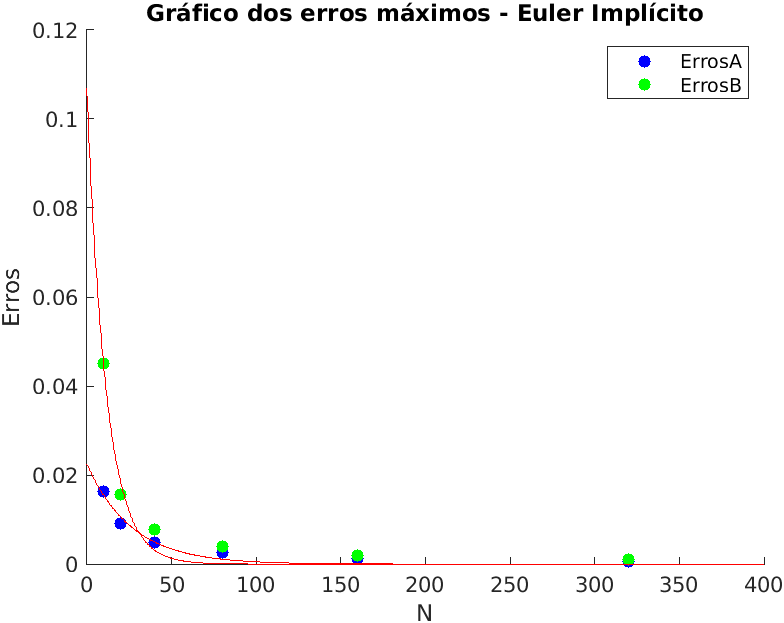
\includegraphics[width=0.65\linewidth]{Segunda_Tarefa/ItemB/erro_euler.png}
    \caption{Ajuste exponencial para os erros}
    \label{fig:2B_Fit_Erro}
\end{figure} 

\subsection{Item C}

O termo de malha para o método de Crank-Nicolson pode ser visto na equação \eqref{crankNicolson}.
\begin{equation} \label{crankNicolson}
u_{i}^{k+1} = u_i^k + \dfrac{\lambda}{2}((u^{k+1}_{i-1} - 2u^{k+1}_{i} + u_{i+1}^{k+1}) + (u^{k}_{i-1} -2u^{k}_i + u^k_{i+1})) + \dfrac{\Delta t}{2}(f(x_i,t_k) + f(x_{i},t_{k+1}))
\end{equation}

Para cada instante de tempo, deve-se resolver o sistema matricial apresentado na equação \eqref{matrix:crank_nicolson}.
\begin{equation}\label{matrix:crank_nicolson}
    \renewcommand*{\arraystretch}{0.75}
    \begin{bmatrix}
    1+\lambda & -\dfrac{\lambda}{2} & 0 & \cdots & 0\\
    -\dfrac{\lambda}{2} & 1+\lambda & -\dfrac{\lambda}{2} & \ddots & \vdots\\
    0 & \ddots & \ddots & \ddots & 0 \\
    \vdots & \ddots & -\dfrac{\lambda}{2} & 1+\lambda & -\dfrac{\lambda}{2} \\
    0 & \cdots & 0 & -\dfrac{\lambda}{2} & 1+\lambda
    \end{bmatrix}
    \begin{bmatrix}
    u_1^{k+1} \\
    u_2^{k+1} \\
    \vdots \\
    u_{N-2}^{k+1} \\
    u_{N-1}^{k+1}
    \end{bmatrix}
    =
\end{equation}
\begin{equation*}
    \begin{bmatrix}
    (1-\lambda)u_1^k + \dfrac{\lambda}{2}(u_0^k + u_2^k) + \dfrac{\Delta t}{2}(f_1^{k}+f_1^{k+1}) + \dfrac{\lambda}{2} g_1(t^{k+1}) \\
    (1-\lambda)u_2^k + \dfrac{\lambda}{2}(u_1^k + u_3^k) + \dfrac{\Delta t}{2}(f_2^{k}+f_2^{k+1}) \\
    \vdots \\
    (1-\lambda)u_{N-2}^k + \dfrac{\lambda}{2}(u_{N-3}^k + u_{N-1}^k) + \dfrac{\Delta t}{2}(f_{N-2}^{k}+f_{N-2}^{k+1}) \\
    (1-\lambda)u_{N-1}^k + \dfrac{\lambda}{2}(u_{N-2}^k + u_{N}^k) + \dfrac{\Delta t}{2}(f_{N-1}^{k}+f_{N-1}^{k+1}) + \dfrac{\lambda}{2} g_2(t^{k+1})
    \end{bmatrix}
\end{equation*}

As soluções encontradas, bem como os erros associados a cada discretização, podem ser vistos nas figuras do apêndice \ref{curvas2C}. Ainda, adotando-se passo temporal de 0,1, traçou-se as curvas das figuras \ref{fig:Tarefa2C_itemA_2D}, \ref{fig:Tarefa2C_itemB_2D} e \ref{fig:Tarefa2C_itemC_2D}. 
\begin{figure}[ht!]
\centering
    \begin{minipage}[b]{0.45\linewidth}
    \includegraphics[width=1\linewidth]{Segunda_Tarefa/ItemC/itemA_2D.png}
    \caption{Solução para o item A, com $N=M=200$}
    \label{fig:Tarefa2C_itemA_2D}
\end{minipage}
\quad
\begin{minipage}[b]{0.45\linewidth}
    \includegraphics[width=1\linewidth]{Segunda_Tarefa/ItemC/itemB_2D.png}
    \caption{Solução para o item B, com $N=M=200$}
    \label{fig:Tarefa2C_itemB_2D}
\end{minipage}
\end{figure}

\begin{figure}[ht!]
    \centering
    \includegraphics[width=0.45\linewidth]{Segunda_Tarefa/ItemC/itemC_2D.png}
    \caption{Solução para o item C, com $N=M=200$}
    \label{fig:Tarefa2C_itemC_2D}
\end{figure}

\clearpage
Observam-se os resultados obtidos, para o método de Crank-Nicolson aplicado ao item C, notam-se oscilações significativas (vide figura \ref{fig:CC_nm10_calculada} do apêndice \ref{curvas2C}). Isso ocorre pois, como visto na figura \ref{fig:fonte_pontual}, a intensidade da fonte apresenta descontinuidade em \textit{p}. 

Nessas condições, lembrando-se que $\lambda > \dfrac{1}{2}$ (considerando que $\Delta x = \Delta t$), o método tende a gerar oscilações espúrias \supercite{osterby}. É de se considerar, portanto, a utilização do método de Euler implícito, o qual é estável e imune à oscilações, para malhas pouco refinadas.

\vspace{1cm}
\begin{figure}[ht]
    \centering
    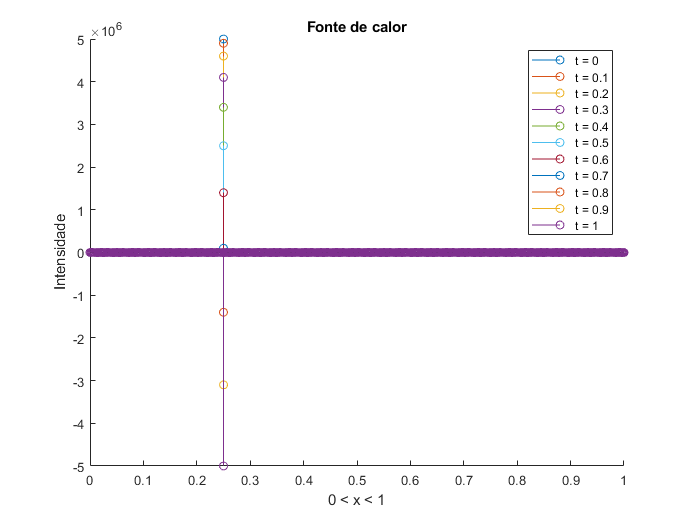
\includegraphics[width=0.8\linewidth]{Segunda_Tarefa/ItemC/fonte.png}
    \caption{Descontinuidade da fonte pontual}
    \label{fig:fonte_pontual}
\end{figure}


O erro máximo, em função de $N$, pode ser visto na figura \ref{fig:2C_Fit_Erro}. Novamente, pode-se observar um fator exponencial de redução para o erro.


\begin{figure}[ht!]
\centering
    \begin{minipage}[b]{0.45\linewidth}
    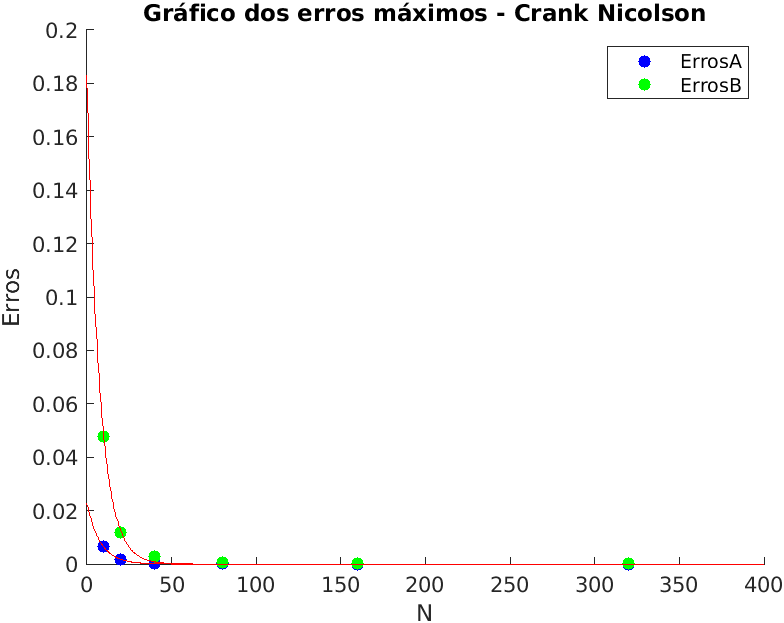
\includegraphics[width=0.95\linewidth]{Segunda_Tarefa/ItemC/erro_crank.png}
    \caption{Ajuste exponencial}
    \label{fig:2C_Fit_Erro}
\end{minipage}
\quad
\begin{minipage}[b]{0.45\linewidth}
    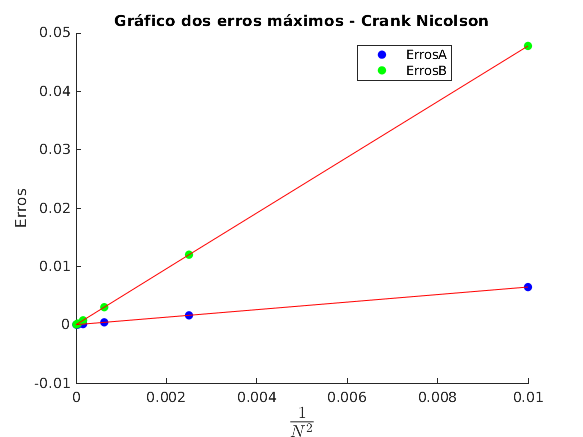
\includegraphics[width=1\linewidth]{Segunda_Tarefa/ItemC/ordem_erro.png}
    \caption{Ordem do erro}
    \label{fig:ordem_erro_CN}
\end{minipage}
\end{figure}

A análise de convergência analítica do método de Crank-Nicolson é complexa. Por essa razão, opta-se pela análise empírica. De acordo com a equação \eqref{erro_proporcional}, pode-se determinar a ordem de convergência de um método a partir da sua relação de proporcionalidade com o passo.

Deve-se verificar que a ordem de convergência do método é 2, então repete-se o gráfico da figura \ref{fig:2C_Fit_Erro}, porém, troca-se a escala do eixo horizontal para o quadrado do passo. Observa-se, na figura \ref{fig:ordem_erro_CN}, que tal relação é linear e, portanto, é possível concluir que o método possui, de fato, convergência de ordem 2 em $\Delta x$ e $\Delta t$.

%----------------------------------------------------------------------------------------%
% Referências 
\clearpage
\addcontentsline{toc}{section}{Referências}
\nocite{begot}
\printbibliography


\newpage
\appendix
\section*{Apêndices}
\addcontentsline{toc}{section}{Apêndices}
\renewcommand{\thesubsection}{\Alph{subsection}}

\subsection{LEIAME} \label{readme}
\vspace{1cm}

\begin{figure}[ht!]
    \centering
    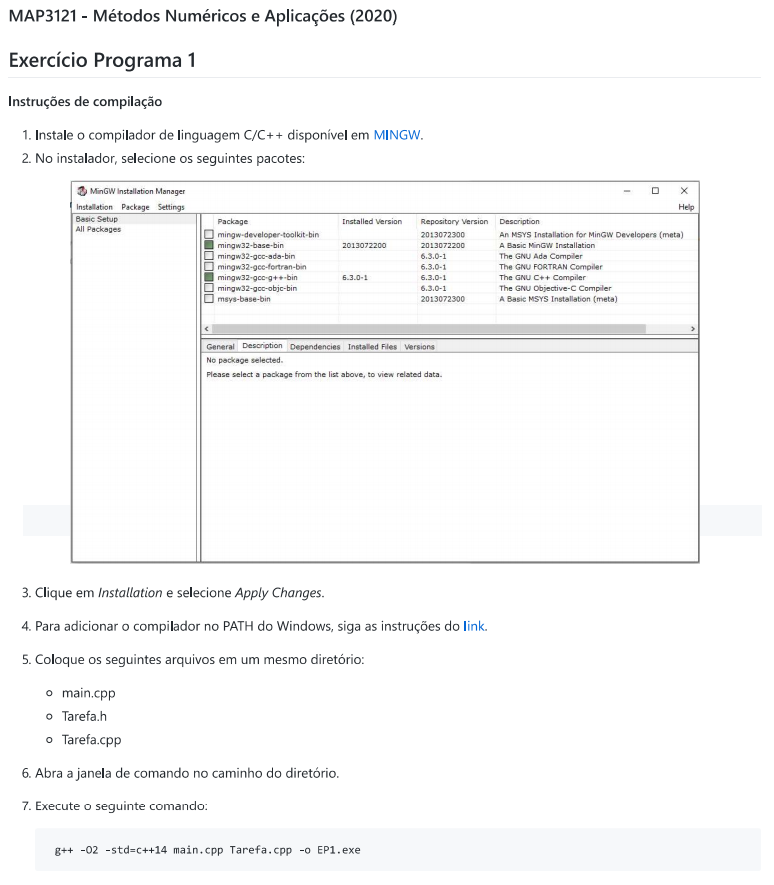
\includegraphics[width=1\linewidth]{README_pg1.png}
    \label{fig:readme_pg1}
\end{figure}

\begin{figure}[ht!]
    \centering
    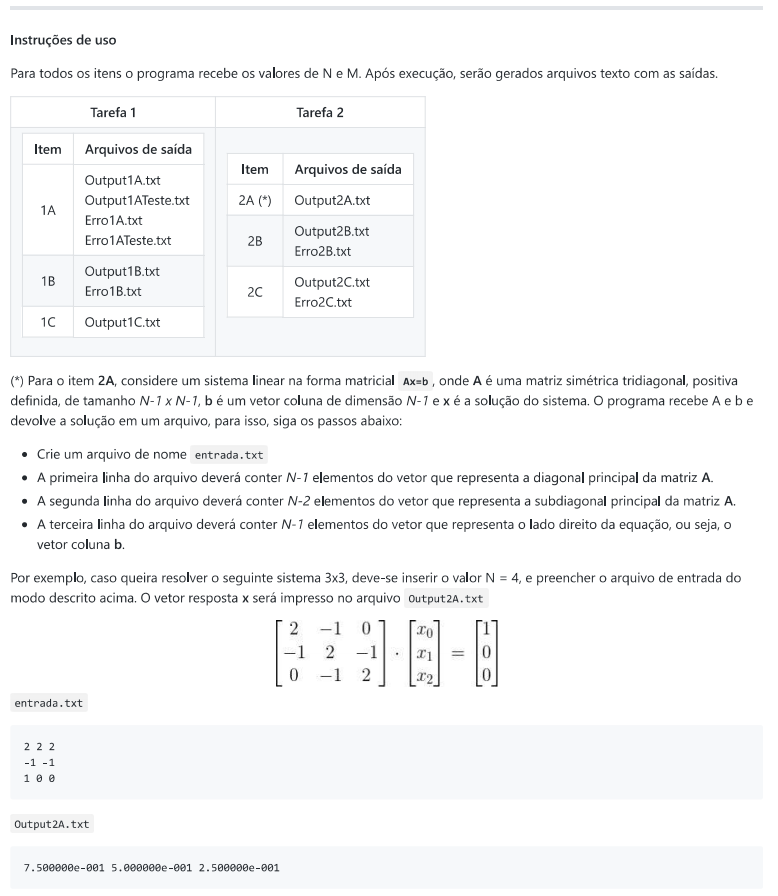
\includegraphics[width=1\linewidth]{README_pg2.png}
    \label{fig:readme_pg2}
\end{figure}

\clearpage
\subsection{Código em MATLAB para gerar as curvas}\label{cod_MATLAB}

\lstinputlisting{Tarefa1.m}
\newpage
\lstinputlisting{Tarefa2.m}


\clearpage
\subsection{Curvas do item 1A} \label{curvas1A}


%------------------- N10 --------------------%

\begin{figure}[ht]
    \centering
    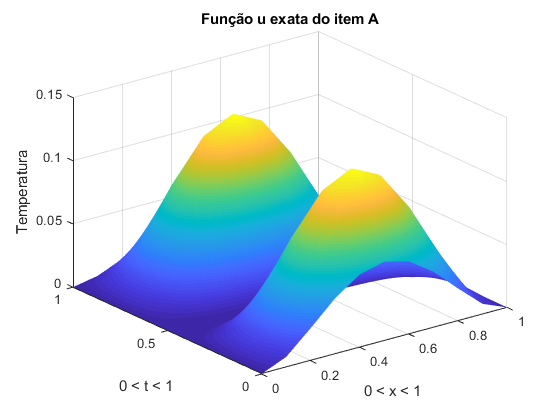
\includegraphics[width=0.8\linewidth]{Primeira_Tarefa/ItemA/n10_lambda0-25_exata.png}
    \caption{Curva da temperatura exata com $N=10$ e $\lambda=0.25$}
    \label{fig:A_n10lambda0-25_exata}
\end{figure}
\begin{figure}
    \centering
    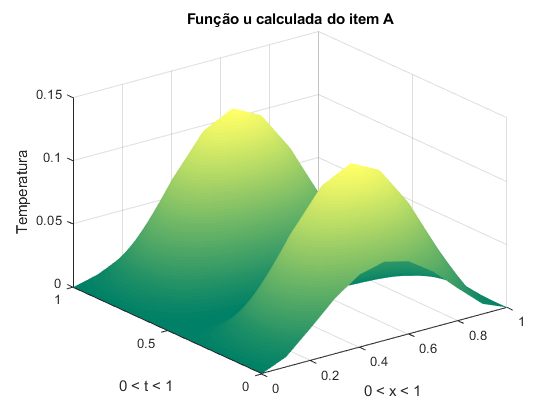
\includegraphics[width=0.8\linewidth]{Primeira_Tarefa/ItemA/n10_lambda0-25_calc.png}
    \caption{Curva da temperatura calculada com $N=10$ e $\lambda=0.5$}
    \label{fig:A_n10lambda0-25_calc}
\end{figure}
\begin{figure}
    \centering
    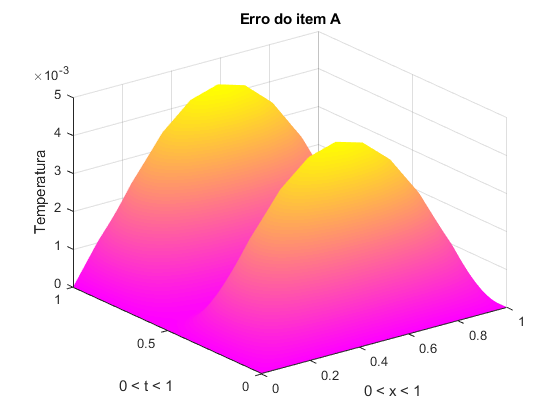
\includegraphics[width=0.8\linewidth]{Primeira_Tarefa/ItemA/n10_lambda0-25_erro.png}
    \caption{Erro com $N=10$ e $\lambda=0.5$}
    \label{fig:A_n10lambda0-25_erro}
\end{figure}
\begin{figure}
    \centering
    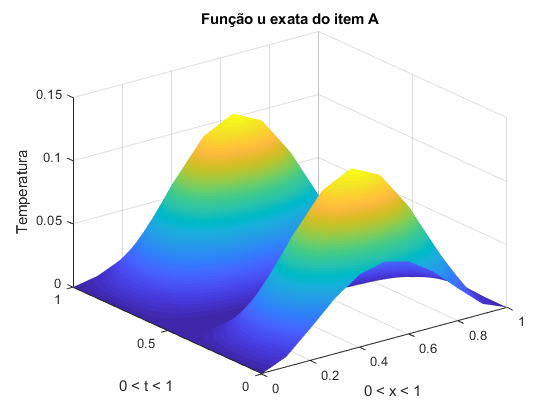
\includegraphics[width=0.8\linewidth]{Primeira_Tarefa/ItemA/n10_lambda0-5_exata.png}
    \caption{Curva da temperatura exata com $N=10$ e $\lambda=0.5$}
    \label{fig:A_n10lambda0-5_exata}
\end{figure}
\begin{figure}
    \centering
    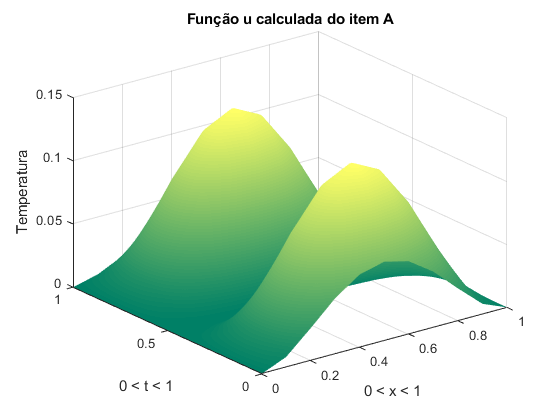
\includegraphics[width=0.8\linewidth]{Primeira_Tarefa/ItemA/n10_lambda0-5_calc.png}
    \caption{Curva da temperatura calculada com $N=10$ e $\lambda=0.5$}
    \label{fig:A_n10lambda0-5_calc}
\end{figure}
\begin{figure}
    \centering
    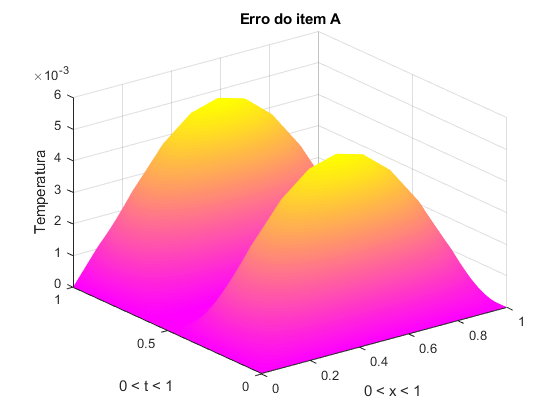
\includegraphics[width=0.8\linewidth]{Primeira_Tarefa/ItemA/n10_lambda0-5_erro.png}
    \caption{Erro com $N=10$ e $\lambda=0.5$}
    \label{fig:A_n10lambda0-5_erro}
\end{figure}

%------------------- N20 --------------------%

\begin{figure}
    \centering
    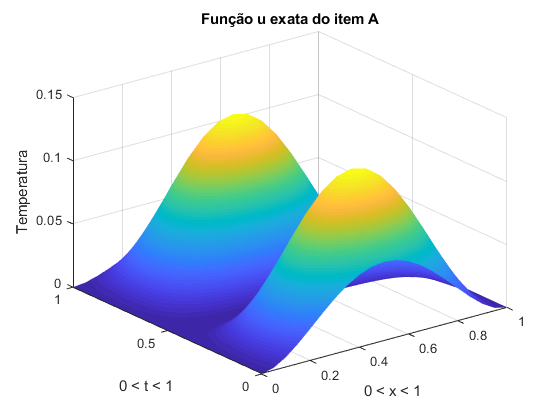
\includegraphics[width=0.8\linewidth]{Primeira_Tarefa/ItemA/n20_lambda0-25_exata.png}
    \caption{Curva da temperatura exata com $N=20$ e $\lambda=0.25$}
    \label{fig:A_n20lambda0-25_exata}
\end{figure}
\begin{figure}
    \centering
    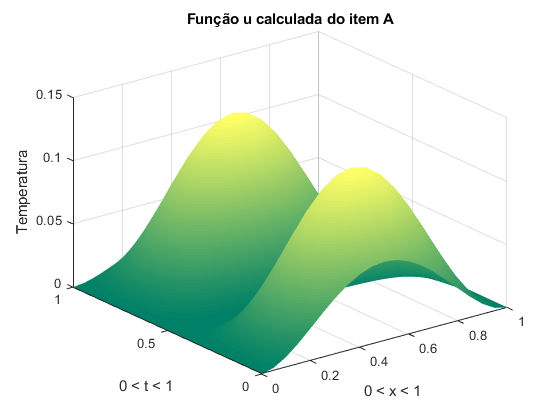
\includegraphics[width=0.8\linewidth]{Primeira_Tarefa/ItemA/n20_lambda0-25_calc.png}
    \caption{Curva da temperatura calculada com $N=20$ e $\lambda=0.25$}
    \label{fig:A_n20lambda0-25_calc}
\end{figure}
\begin{figure}
    \centering
    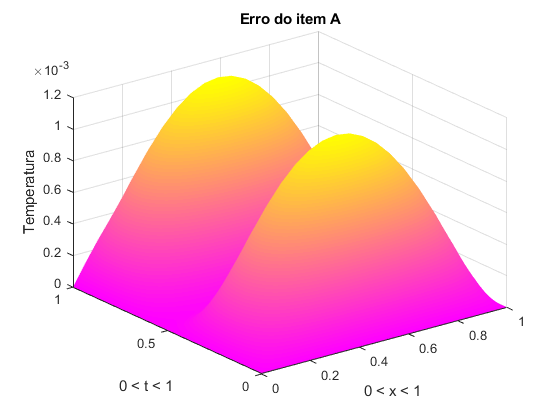
\includegraphics[width=0.8\linewidth]{Primeira_Tarefa/ItemA/n20_lambda0-25_erro.png}
    \caption{Erro com $N=20$ e $\lambda=0.25$}
    \label{fig:A_n20lambda0-25_erro}
\end{figure}
\begin{figure}
    \centering
    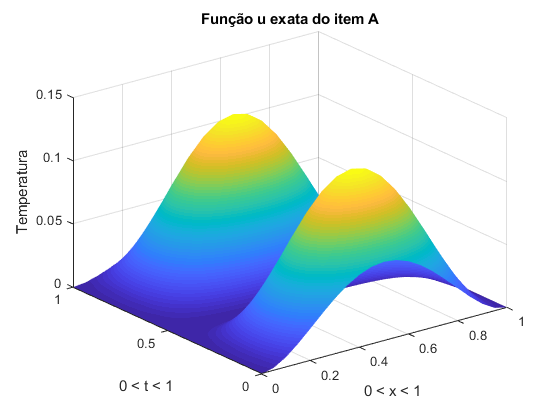
\includegraphics[width=0.8\linewidth]{Primeira_Tarefa/ItemA/n20_lambda0-5_exata.png}
    \caption{Curva da temperatura exata com $N=20$ e $\lambda=0.5$}
    \label{fig:A_n20lambda0-5_exata}
\end{figure}
\begin{figure}
    \centering
    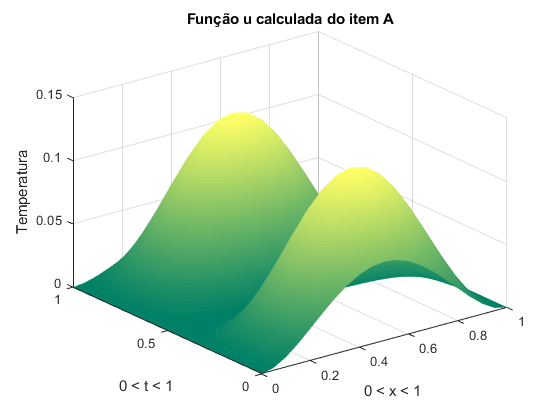
\includegraphics[width=0.8\linewidth]{Primeira_Tarefa/ItemA/n20_lambda0-5_calc.png}
    \caption{Curva da temperatura calculada com $N=20$ e $\lambda=0.5$}
    \label{fig:A_n20lambda0-5_calc}
\end{figure}
\begin{figure}
    \centering
    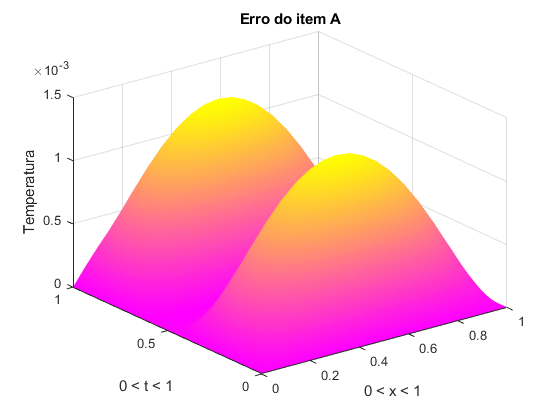
\includegraphics[width=0.8\linewidth]{Primeira_Tarefa/ItemA/n20_lambda0-5_erro.png}
    \caption{Erro com $N=20$ e $\lambda=0.5$}
    \label{fig:A_n20lambda0-5_erro}
\end{figure}

%------------------- N40 --------------------%

\begin{figure}
    \centering
    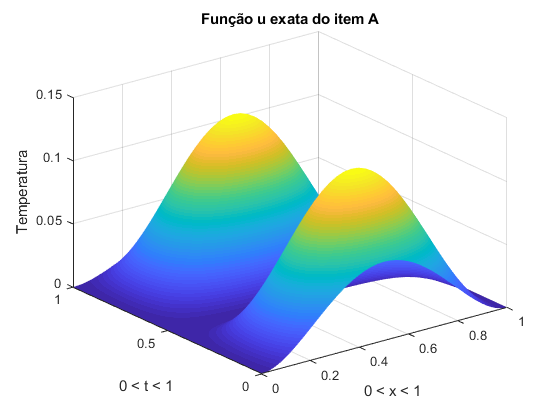
\includegraphics[width=0.8\linewidth]{Primeira_Tarefa/ItemA/n40_lambda0-25_exata.png}
    \caption{Curva da temperatura exata com $N=40$ e $\lambda=0.25$}
    \label{fig:A_n40lambda0-25_exata}
\end{figure}
\begin{figure}
    \centering
    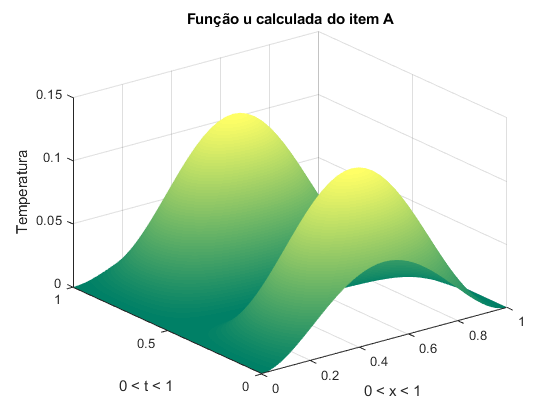
\includegraphics[width=0.8\linewidth]{Primeira_Tarefa/ItemA/n40_lambda0-25_calc.png}
    \caption{Curva da temperatura calculada com $N=40$ e $\lambda=0.25$}
    \label{fig:A_n40lambda0-25_calc}
\end{figure}
\begin{figure}
    \centering
    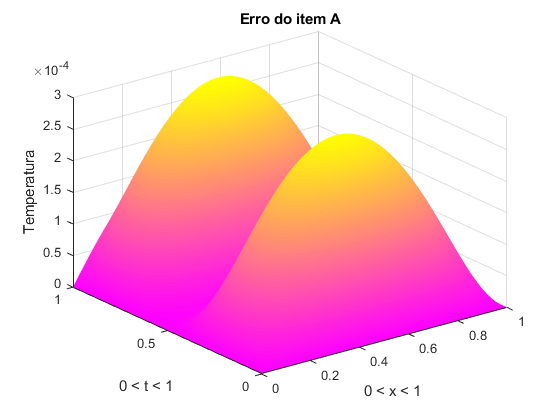
\includegraphics[width=0.8\linewidth]{Primeira_Tarefa/ItemA/n40_lambda0-25_erro.png}
    \caption{Erro com $N=40$ e $\lambda=0.25$}
    \label{fig:A_n40lambda0-25_erro}
\end{figure}
\begin{figure}
    \centering
    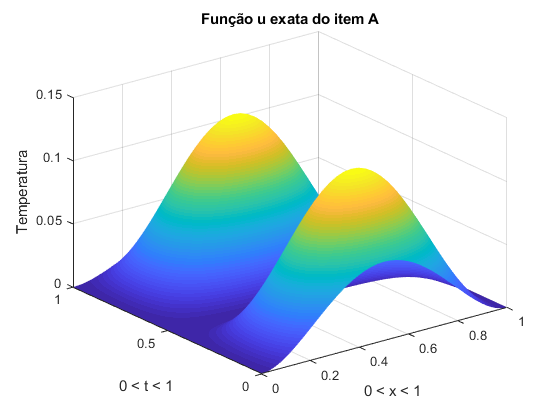
\includegraphics[width=0.8\linewidth]{Primeira_Tarefa/ItemA/n40_lambda0-5_exata.png}
    \caption{Curva da temperatura exata com $N=40$ e $\lambda=0.5$}
    \label{fig:A_n40lambda0-5_exata}
\end{figure}
\begin{figure}
    \centering
    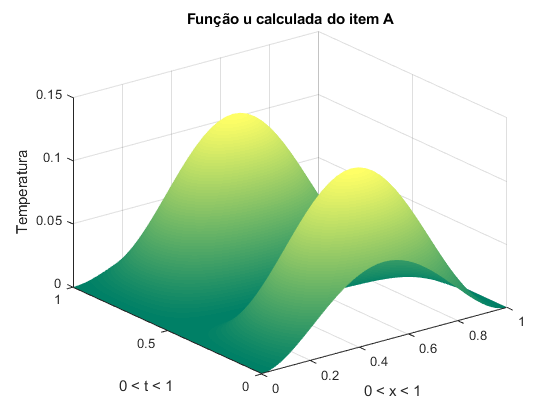
\includegraphics[width=0.8\linewidth]{Primeira_Tarefa/ItemA/n40_lambda0-5_calc.png}
    \caption{Curva da temperatura calculada com $N=40$ e $\lambda=0.5$}
    \label{fig:A_n40lambda0-5_calc}
\end{figure}
\begin{figure}
    \centering
    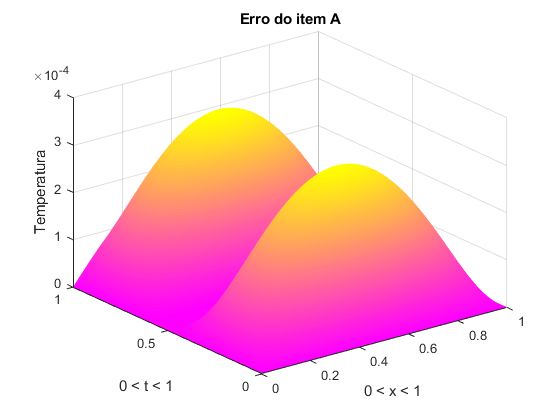
\includegraphics[width=0.8\linewidth]{Primeira_Tarefa/ItemA/n40_lambda0-5_erro.png}
    \caption{Erro com $N=40$ e $\lambda=0.5$}
    \label{fig:A_n40lambda0-5_erro}
\end{figure}

%------------------- N80 --------------------%

\begin{figure}
    \centering
    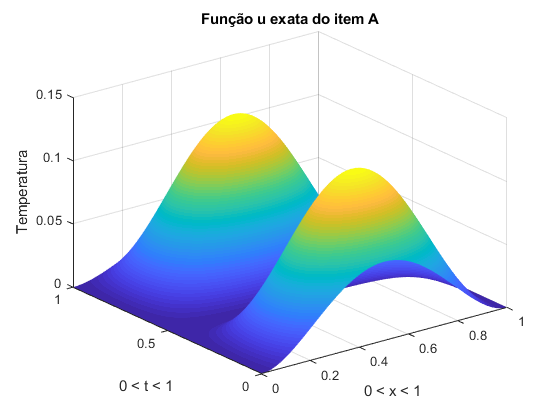
\includegraphics[width=0.8\linewidth]{Primeira_Tarefa/ItemA/n80_lambda0-25_exata.png}
    \caption{Curva da temperatura exata com $N=80$ e $\lambda=0.25$}
    \label{fig:A_n80lambda0-25_exata}
\end{figure}
\begin{figure}
    \centering
    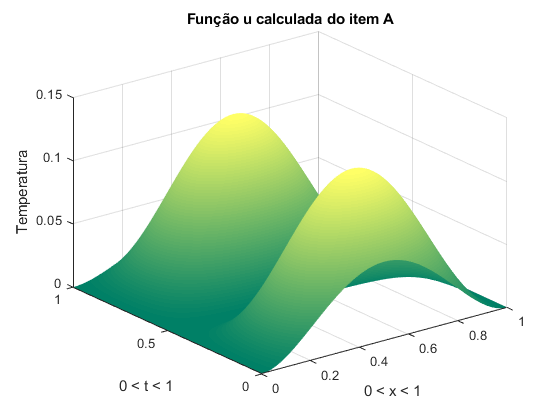
\includegraphics[width=0.8\linewidth]{Primeira_Tarefa/ItemA/n80_lambda0-25_calc.png}
    \caption{Curva da temperatura calculada com $N=80$ e $\lambda=0.25$}
    \label{fig:A_n80lambda0-25_calc}
\end{figure}
\begin{figure}
    \centering
    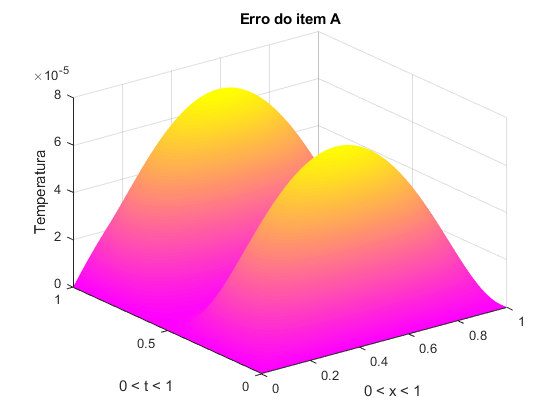
\includegraphics[width=0.8\linewidth]{Primeira_Tarefa/ItemA/n80_lambda0-25_erro.png}
    \caption{Erro com $N=80$ e $\lambda=0.25$}
    \label{fig:A_n80lambda0-25_erro}
\end{figure}
\begin{figure}
    \centering
    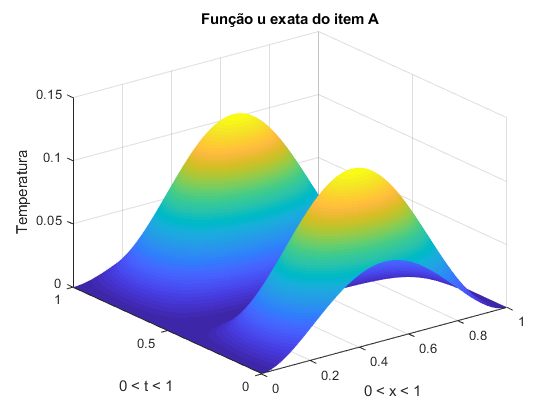
\includegraphics[width=0.8\linewidth]{Primeira_Tarefa/ItemA/n80_lambda0-5_exata.png}
    \caption{Curva da temperatura exata com $N=80$ e $\lambda=0.5$}
    \label{fig:A_n80lambda0-5_exata}
\end{figure}
\begin{figure}
    \centering
    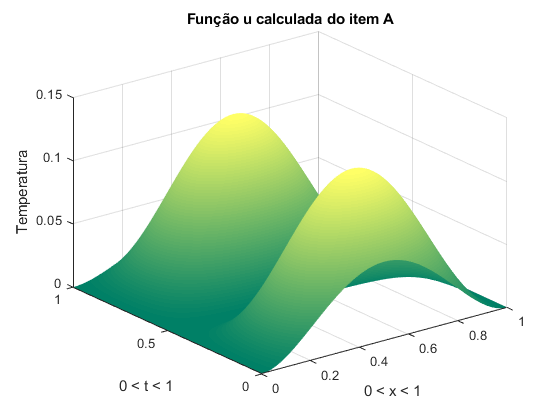
\includegraphics[width=0.8\linewidth]{Primeira_Tarefa/ItemA/n80_lambda0-5_calc.png}
    \caption{Curva da temperatura calculada com $N=80$ e $\lambda=0.5$}
    \label{fig:A_n80lambda0-5_calc}
\end{figure}
\begin{figure}
    \centering
    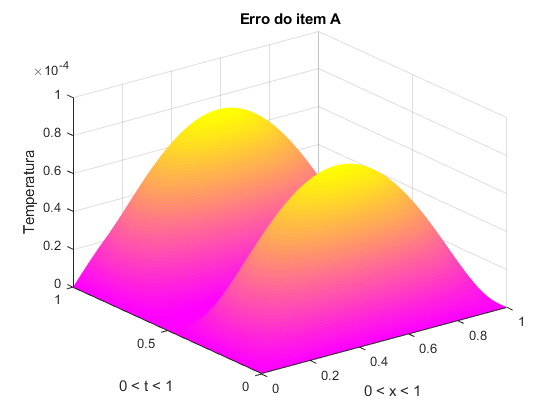
\includegraphics[width=0.8\linewidth]{Primeira_Tarefa/ItemA/n80_lambda0-5_erro.png}
    \caption{Erro com $N=80$ e $\lambda=0.5$}
    \label{fig:A_n80lambda0-5_erro}
\end{figure}

%------------------- N160 --------------------%

\begin{figure}
    \centering
    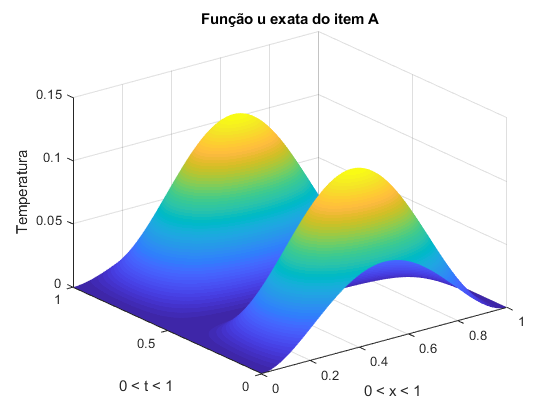
\includegraphics[width=0.8\linewidth]{Primeira_Tarefa/ItemA/n160_lambda0-25_exata.png}
    \caption{Curva da temperatura exata com $N=160$ e $\lambda=0.25$}
    \label{fig:A_n160lambda0-25_exata}
\end{figure}
\begin{figure}
    \centering
    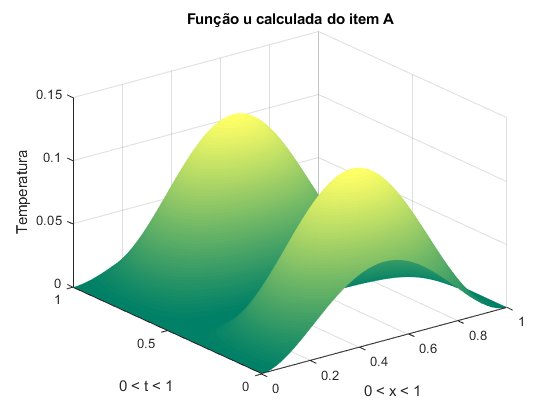
\includegraphics[width=0.8\linewidth]{Primeira_Tarefa/ItemA/n160_lambda0-25_calc.png}
    \caption{Curva da temperatura calculada com $N=160$ e $\lambda=0.25$}
    \label{fig:A_n160lambda0-25_calc}
\end{figure}
\begin{figure}
    \centering
    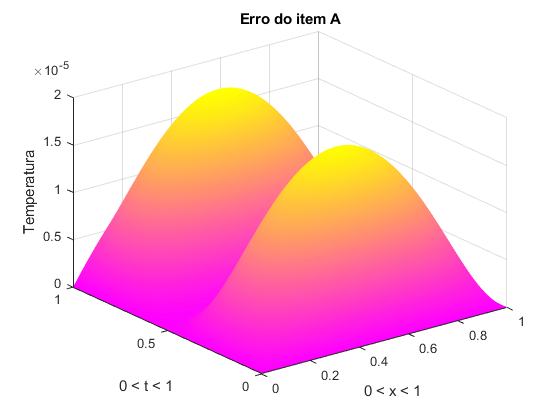
\includegraphics[width=0.8\linewidth]{Primeira_Tarefa/ItemA/n160_lambda0-25_erro.png}
    \caption{Erro com $N=160$ e $\lambda=0.25$}
    \label{fig:A_n160lambda0-25_erro}
\end{figure}
\begin{figure}
    \centering
    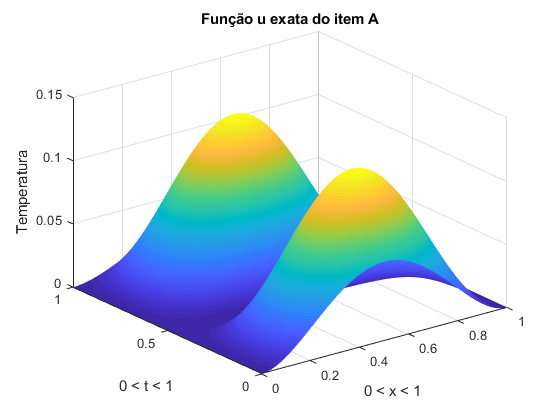
\includegraphics[width=0.8\linewidth]{Primeira_Tarefa/ItemA/n160_lambda0-5_exata.png}
    \caption{Curva da temperatura exata com $N=160$ e $\lambda=0.5$}
    \label{fig:A_n160lambda0-5_exata}
\end{figure}
\begin{figure}
    \centering
    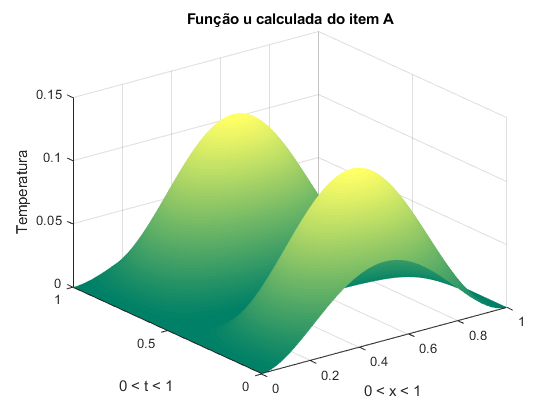
\includegraphics[width=0.8\linewidth]{Primeira_Tarefa/ItemA/n160_lambda0-5_calc.png}
    \caption{Curva da temperatura calculada com $N=160$ e $\lambda=0.5$}
    \label{fig:A_n160lambda0-5_calc}
\end{figure}
\begin{figure}
    \centering
    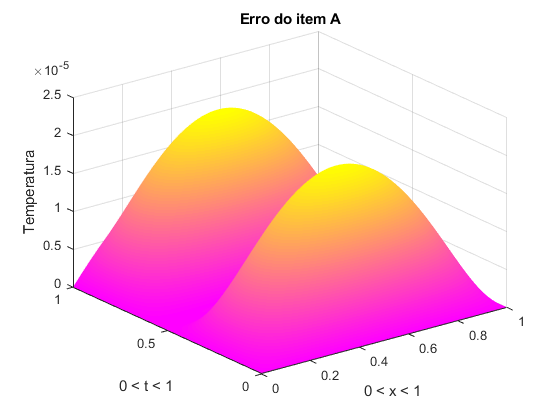
\includegraphics[width=0.8\linewidth]{Primeira_Tarefa/ItemA/n160_lambda0-5_erro.png}
    \caption{Erro com $N=160$ e $\lambda=0.5$}
    \label{fig:A_n160lambda0-5_erro}
\end{figure}

%------------------- N320 --------------------%

\begin{figure}
    \centering
    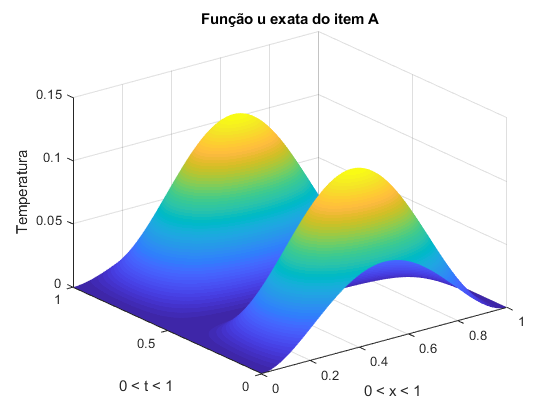
\includegraphics[width=0.8\linewidth]{Primeira_Tarefa/ItemA/n320_lambda0-25_exata.png}
    \caption{Curva da temperatura exata com $N=320$ e $\lambda=0.25$}
    \label{fig:A_n320lambda0-25_exata}
\end{figure}
\begin{figure}
    \centering
    \includegraphics[width=0.8\linewidth]{Primeira_Tarefa/ItemA/n320_lambda0-25_calc.png}
    \caption{Curva da temperatura calculada com $N=320$ e $\lambda=0.25$}
    \label{fig:A_n320lambda0-25_calc}
\end{figure}
\begin{figure}
    \centering
    \includegraphics[width=0.8\linewidth]{Primeira_Tarefa/ItemA/n320_lambda0-25_erro.png}
    \caption{Erro com $N=320$ e $\lambda=0.25$}
    \label{fig:A_n320lambda0-25_erro}
\end{figure}
\begin{figure}
    \centering
    \includegraphics[width=0.8\linewidth]{Primeira_Tarefa/ItemA/n320_lambda0-5_exata.png}
    \caption{Curva da temperatura exata com $N=320$ e $\lambda=0.5$}
    \label{fig:A_n320lambda0-5_exata}
\end{figure}
\begin{figure}
    \centering
    \includegraphics[width=0.8\linewidth]{Primeira_Tarefa/ItemA/n320_lambda0-5_calc.png}
    \caption{Curva da temperatura calculada com $N=320$ e $\lambda=0.5$}
    \label{fig:A_n320lambda0-5_calc}
\end{figure}
\begin{figure}
    \centering
    \includegraphics[width=0.8\linewidth]{Primeira_Tarefa/ItemA/n320_lambda0-5_erro.png}
    \caption{Erro com $N=320$ e $\lambda=0.5$}
    \label{fig:A_n320lambda0-5_erro}
\end{figure}


\clearpage
\subsection{Curvas do item 1B} \label{curvas1B}

\begin{figure}[ht!]
    \centering
    \includegraphics[width=0.8\linewidth]{Primeira_Tarefa/ItemB/n10_lambda0-25_exata.png}
    \caption{Curva da temperatura exata com $N=10$ e $\lambda=0.25$}
    \label{fig:B_n10lambda0-25_exata}
\end{figure}
\begin{figure}
    \centering
    \includegraphics[width=0.8\linewidth]{Primeira_Tarefa/ItemB/n10_lambda0-25_calc.png}
    \caption{Curva da temperatura calculada com $N=10$ e $\lambda=0.5$}
    \label{fig:B_n10lambda0-25_calc}
\end{figure}
\begin{figure}
    \centering
    \includegraphics[width=0.8\linewidth]{Primeira_Tarefa/ItemB/n10_lambda0-25_erro.png}
    \caption{Erro com $N=10$ e $\lambda=0.5$}
    \label{fig:B_n10lambda0-25_erro}
\end{figure}
\begin{figure}
    \centering
    \includegraphics[width=0.8\linewidth]{Primeira_Tarefa/ItemB/n10_lambda0-5_exata.png}
    \caption{Curva da temperatura exata com $N=10$ e $\lambda=0.5$}
    \label{fig:B_n10lambda0-5_exata}
\end{figure}
\begin{figure}
    \centering
    \includegraphics[width=0.8\linewidth]{Primeira_Tarefa/ItemB/n10_lambda0-5_calc.png}
    \caption{Curva da temperatura calculada com $N=10$ e $\lambda=0.5$}
    \label{fig:B_n10lambda0-5_calc}
\end{figure}
\begin{figure}
    \centering
    \includegraphics[width=0.8\linewidth]{Primeira_Tarefa/ItemB/n10_lambda0-5_erro.png}
    \caption{Erro com $N=10$ e $\lambda=0.5$}
    \label{fig:B_n10lambda0-5_erro}
\end{figure}

%------------------- N20 --------------------%

\begin{figure}
    \centering
    \includegraphics[width=0.8\linewidth]{Primeira_Tarefa/ItemB/n20_lambda0-25_exata.png}
    \caption{Curva da temperatura exata com $N=20$ e $\lambda=0.25$}
    \label{fig:B_n20lambda0-25_exata}
\end{figure}
\begin{figure}
    \centering
    \includegraphics[width=0.8\linewidth]{Primeira_Tarefa/ItemB/n20_lambda0-25_calc.png}
    \caption{Curva da temperatura calculada com $N=20$ e $\lambda=0.25$}
    \label{fig:B_n20lambda0-25_calc}
\end{figure}
\begin{figure}
    \centering
    \includegraphics[width=0.8\linewidth]{Primeira_Tarefa/ItemB/n20_lambda0-25_erro.png}
    \caption{Erro com $N=20$ e $\lambda=0.25$}
    \label{fig:B_n20lambda0-25_erro}
\end{figure}
\begin{figure}
    \centering
    \includegraphics[width=0.8\linewidth]{Primeira_Tarefa/ItemB/n20_lambda0-5_exata.png}
    \caption{Curva da temperatura exata com $N=20$ e $\lambda=0.5$}
    \label{fig:B_n20lambda0-5_exata}
\end{figure}
\begin{figure}
    \centering
    \includegraphics[width=0.8\linewidth]{Primeira_Tarefa/ItemB/n20_lambda0-5_calc.png}
    \caption{Curva da temperatura calculada com $N=20$ e $\lambda=0.5$}
    \label{fig:B_n20lambda0-5_calc}
\end{figure}
\begin{figure}
    \centering
    \includegraphics[width=0.8\linewidth]{Primeira_Tarefa/ItemB/n20_lambda0-5_erro.png}
    \caption{Erro com $N=20$ e $\lambda=0.5$}
    \label{fig:B_n20lambda0-5_erro}
\end{figure}

%------------------- N40 --------------------%

\begin{figure}
    \centering
    \includegraphics[width=0.8\linewidth]{Primeira_Tarefa/ItemB/n40_lambda0-25_exata.png}
    \caption{Curva da temperatura exata com $N=40$ e $\lambda=0.25$}
    \label{fig:B_n40lambda0-25_exata}
\end{figure}
\begin{figure}
    \centering
    \includegraphics[width=0.8\linewidth]{Primeira_Tarefa/ItemB/n40_lambda0-25_calc.png}
    \caption{Curva da temperatura calculada com $N=40$ e $\lambda=0.25$}
    \label{fig:B_n40lambda0-25_calc}
\end{figure}
\begin{figure}
    \centering
    \includegraphics[width=0.8\linewidth]{Primeira_Tarefa/ItemB/n40_lambda0-25_erro.png}
    \caption{Erro com $N=40$ e $\lambda=0.25$}
    \label{fig:B_n40lambda0-25_erro}
\end{figure}
\begin{figure}
    \centering
    \includegraphics[width=0.8\linewidth]{Primeira_Tarefa/ItemB/n40_lambda0-5_exata.png}
    \caption{Curva da temperatura exata com $N=40$ e $\lambda=0.5$}
    \label{fig:B_n40lambda0-5_exata}
\end{figure}
\begin{figure}
    \centering
    \includegraphics[width=0.8\linewidth]{Primeira_Tarefa/ItemB/n40_lambda0-5_calc.png}
    \caption{Curva da temperatura calculada com $N=40$ e $\lambda=0.5$}
    \label{fig:B_n40lambda0-5_calc}
\end{figure}
\begin{figure}
    \centering
    \includegraphics[width=0.8\linewidth]{Primeira_Tarefa/ItemB/n40_lambda0-5_erro.png}
    \caption{Erro com $N=40$ e $\lambda=0.5$}
    \label{fig:B_n40lambda0-5_erro}
\end{figure}

%------------------- N80 --------------------%

\begin{figure}
    \centering
    \includegraphics[width=0.8\linewidth]{Primeira_Tarefa/ItemB/n80_lambda0-25_exata.png}
    \caption{Curva da temperatura exata com $N=80$ e $\lambda=0.25$}
    \label{fig:B_n80lambda0-25_exata}
\end{figure}
\begin{figure}
    \centering
    \includegraphics[width=0.8\linewidth]{Primeira_Tarefa/ItemB/n80_lambda0-25_calc.png}
    \caption{Curva da temperatura calculada com $N=80$ e $\lambda=0.25$}
    \label{fig:B_n80lambda0-25_calc}
\end{figure}
\begin{figure}
    \centering
    \includegraphics[width=0.8\linewidth]{Primeira_Tarefa/ItemB/n80_lambda0-25_erro.png}
    \caption{Erro com $N=80$ e $\lambda=0.25$}
    \label{fig:B_n80lambda0-25_erro}
\end{figure}
\begin{figure}
    \centering
    \includegraphics[width=0.8\linewidth]{Primeira_Tarefa/ItemB/n80_lambda0-5_exata.png}
    \caption{Curva da temperatura exata com $N=80$ e $\lambda=0.5$}
    \label{fig:B_n80lambda0-5_exata}
\end{figure}
\begin{figure}
    \centering
    \includegraphics[width=0.8\linewidth]{Primeira_Tarefa/ItemB/n80_lambda0-5_calc.png}
    \caption{Curva da temperatura calculada com $N=80$ e $\lambda=0.5$}
    \label{fig:B_n80lambda0-5_calc}
\end{figure}
\begin{figure}
    \centering
    \includegraphics[width=0.8\linewidth]{Primeira_Tarefa/ItemB/n80_lambda0-5_erro.png}
    \caption{Erro com $N=80$ e $\lambda=0.5$}
    \label{fig:B_n80lambda0-5_erro}
\end{figure}

%------------------- N160 --------------------%

\begin{figure}
    \centering
    \includegraphics[width=0.8\linewidth]{Primeira_Tarefa/ItemB/n160_lambda0-25_exata.png}
    \caption{Curva da temperatura exata com $N=160$ e $\lambda=0.25$}
    \label{fig:B_n160lambda0-25_exata}
\end{figure}
\begin{figure}
    \centering
    \includegraphics[width=0.8\linewidth]{Primeira_Tarefa/ItemB/n160_lambda0-25_calc.png}
    \caption{Curva da temperatura calculada com $N=160$ e $\lambda=0.25$}
    \label{fig:B_n160lambda0-25_calc}
\end{figure}
\begin{figure}
    \centering
    \includegraphics[width=0.8\linewidth]{Primeira_Tarefa/ItemB/n160_lambda0-25_erro.png}
    \caption{Erro com $N=160$ e $\lambda=0.25$}
    \label{fig:B_n160lambda0-25_erro}
\end{figure}
\begin{figure}
    \centering
    \includegraphics[width=0.8\linewidth]{Primeira_Tarefa/ItemB/n160_lambda0-5_exata.png}
    \caption{Curva da temperatura exata com $N=160$ e $\lambda=0.5$}
    \label{fig:B_n160lambda0-5_exata}
\end{figure}
\begin{figure}
    \centering
    \includegraphics[width=0.8\linewidth]{Primeira_Tarefa/ItemB/n160_lambda0-5_calc.png}
    \caption{Curva da temperatura calculada com $N=160$ e $\lambda=0.5$}
    \label{fig:B_n160lambda0-5_calc}
\end{figure}
\begin{figure}
    \centering
    \includegraphics[width=0.8\linewidth]{Primeira_Tarefa/ItemB/n160_lambda0-5_erro.png}
    \caption{Erro com $N=160$ e $\lambda=0.5$}
    \label{fig:B_n160lambda0-5_erro}
\end{figure}

%------------------- N320 --------------------%

\begin{figure}
    \centering
    \includegraphics[width=0.8\linewidth]{Primeira_Tarefa/ItemB/n320_lambda0-25_exata.png}
    \caption{Curva da temperatura exata com $N=320$ e $\lambda=0.25$}
    \label{fig:B_n320lambda0-25_exata}
\end{figure}
\begin{figure}
    \centering
    \includegraphics[width=0.8\linewidth]{Primeira_Tarefa/ItemB/n320_lambda0-25_calc.png}
    \caption{Curva da temperatura calculada com $N=320$ e $\lambda=0.25$}
    \label{fig:B_n320lambda0-25_calc}
\end{figure}
\begin{figure}
    \centering
    \includegraphics[width=0.8\linewidth]{Primeira_Tarefa/ItemB/n320_lambda0-25_erro.png}
    \caption{Erro com $N=320$ e $\lambda=0.25$}
    \label{fig:B_n320lambda0-25_erro}
\end{figure}
\begin{figure}
    \centering
    \includegraphics[width=0.8\linewidth]{Primeira_Tarefa/ItemB/n320_lambda0-5_exata.png}
    \caption{Curva da temperatura exata com $N=320$ e $\lambda=0.5$}
    \label{fig:B_n320lambda0-5_exata}
\end{figure}
\begin{figure}
    \centering
    \includegraphics[width=0.8\linewidth]{Primeira_Tarefa/ItemB/n320_lambda0-5_calc.png}
    \caption{Curva da temperatura calculada com $N=320$ e $\lambda=0.5$}
    \label{fig:B_n320lambda0-5_calc}
\end{figure}
\begin{figure}
    \centering
    \includegraphics[width=0.8\linewidth]{Primeira_Tarefa/ItemB/n320_lambda0-5_erro.png}
    \caption{Erro com $N=320$ e $\lambda=0.5$}
    \label{fig:B_n320lambda0-5_erro}
\end{figure}


\clearpage
\subsection{Curvas do item 1C} \label{curvas1C}

%------------------- N10 --------------------%

\begin{figure}[ht!]
    \centering
    \includegraphics[width=0.8\linewidth]{Primeira_Tarefa/ItemC/n10_lambda0-25_calc.png}
    \caption{Curva da temperatura calculada com $N=10$ e $\lambda=0.25$}
    \label{fig:C_n10lambda0-25_exata}
\end{figure}
\begin{figure}
    \centering
    \includegraphics[width=0.8\linewidth]{Primeira_Tarefa/ItemC/n10_lambda0-5_calc.png}
    \caption{Curva da temperatura calculada com $N=10$ e $\lambda=0.5$}
    \label{fig:C_n10lambda0-5_calc}
\end{figure}

%------------------- N20 --------------------%

\begin{figure}
    \centering
    \includegraphics[width=0.8\linewidth]{Primeira_Tarefa/ItemC/n20_lambda0-25_calc.png}
    \caption{Curva da temperatura exata com $N=20$ e $\lambda=0.25$}
    \label{fig:C_n20lambda0-25_exata}
\end{figure}
\begin{figure}
    \centering
    \includegraphics[width=0.8\linewidth]{Primeira_Tarefa/ItemC/n20_lambda0-5_calc.png}
    \caption{Curva da temperatura calculada com $N=20$ e $\lambda=0.5$}
    \label{fig:C_n20lambda0-5_calc}
\end{figure}

%------------------- N40 --------------------%

\begin{figure}
    \centering
    \includegraphics[width=0.8\linewidth]{Primeira_Tarefa/ItemC/n40_lambda0-25_calc.png}
    \caption{Curva da temperatura calculada com $N=40$ e $\lambda=0.25$}
    \label{fig:C_n40lambda0-25_calc}
\end{figure}
\begin{figure}
    \centering
    \includegraphics[width=0.8\linewidth]{Primeira_Tarefa/ItemC/n40_lambda0-5_calc.png}
    \caption{Curva da temperatura calculada com $N=40$ e $\lambda=0.5$}
    \label{fig:C_n40lambda0-5_calc}
\end{figure}

%------------------- N80 --------------------%

\begin{figure}
    \centering
    \includegraphics[width=0.8\linewidth]{Primeira_Tarefa/ItemC/n80_lambda0-25_calc.png}
    \caption{Curva da temperatura calculada com $N=80$ e $\lambda=0.25$}
    \label{fig:C_n80lambda0-25_exata}
\end{figure}
\begin{figure}
    \centering
    \includegraphics[width=0.8\linewidth]{Primeira_Tarefa/ItemC/n80_lambda0-5_calc.png}
    \caption{Curva da temperatura calculada com $N=80$ e $\lambda=0.5$}
    \label{fig:C_n80lambda0-5_calc}
\end{figure}

%------------------- N160 --------------------%

\begin{figure}
    \centering
    \includegraphics[width=0.8\linewidth]{Primeira_Tarefa/ItemC/n160_lambda0-25_calc.png}
    \caption{Curva da temperatura calculada com $N=160$ e $\lambda=0.25$}
    \label{fig:C_n160lambda0-25_exata}
\end{figure}
\begin{figure}
    \centering
    \includegraphics[width=0.8\linewidth]{Primeira_Tarefa/ItemC/n160_lambda0-5_calc.png}
    \caption{Curva da temperatura calculada com $N=160$ e $\lambda=0.5$}
    \label{fig:C_n160lambda0-5_calc}
\end{figure}

%------------------- N320 --------------------%

\begin{figure}
    \centering
    \includegraphics[width=0.8\linewidth]{Primeira_Tarefa/ItemC/n320_lambda0-25_calc.png}
    \caption{Curva da temperatura calculada com $N=320$ e $\lambda=0.25$}
    \label{fig:C_n320lambda0-25_exata}
\end{figure}
\begin{figure}
    \centering
    \includegraphics[width=0.8\linewidth]{Primeira_Tarefa/ItemC/n320_lambda0-5_calc.png}
    \caption{Curva da temperatura calculada com $N=320$ e $\lambda=0.5$}
    \label{fig:C_n320lambda0-5_calc}
\end{figure}

%------------------- 2B --------------------%

\clearpage
\subsection{Curvas do item 2B} \label{curvas2B}

\begin{figure}[ht!]
    \centering
    \includegraphics[width=0.8\linewidth]{Segunda_Tarefa/ItemB/nm10_calculada_A.png}
    \caption{Curva da temperatura calculada com $N=M=10$}
    \label{fig:BA_nm10_calculada}
\end{figure}

\begin{figure}
    \centering
    \includegraphics[width=0.8\linewidth]{Segunda_Tarefa/ItemB/nm10_erro_A.png}
    \caption{Erro com $N=M=10$}
    \label{fig:BA_nm10_erro}
\end{figure}

\begin{figure}
    \centering
    \includegraphics[width=0.8\linewidth]{Segunda_Tarefa/ItemB/nm20_calculada_A.png}
    \caption{Curva da temperatura calculada com $N=M=20$}
    \label{fig:BA_nm20_calculada}
\end{figure}

\begin{figure}
    \centering
    \includegraphics[width=0.8\linewidth]{Segunda_Tarefa/ItemB/nm20_erro_A.png}
    \caption{Erro com $N=M=20$}
    \label{fig:BA_nm20_erro}
\end{figure}

\begin{figure}
    \centering
    \includegraphics[width=0.8\linewidth]{Segunda_Tarefa/ItemB/nm40_calculada_A.png}
    \caption{Curva da temperatura calculada com $N=M=40$}
    \label{fig:BA_nm40_calculada}
\end{figure}

\begin{figure}
    \centering
    \includegraphics[width=0.8\linewidth]{Segunda_Tarefa/ItemB/nm40_erro_A.png}
    \caption{Erro com $N=M=40$}
    \label{fig:BA_nm40_erro}
\end{figure}

\begin{figure}
    \centering
    \includegraphics[width=0.8\linewidth]{Segunda_Tarefa/ItemB/nm80_calculada_A.png}
    \caption{Curva da temperatura calculada com $N=M=80$}
    \label{fig:BA_nm80_calculada}
\end{figure}

\begin{figure}
    \centering
    \includegraphics[width=0.8\linewidth]{Segunda_Tarefa/ItemB/nm80_erro_A.png}
    \caption{Erro com $N=M=80$}
    \label{fig:BA_nm80_erro}
\end{figure}

\begin{figure}
    \centering
    \includegraphics[width=0.8\linewidth]{Segunda_Tarefa/ItemB/nm160_calculada_A.png}
    \caption{Curva da temperatura calculada com $N=M=160$}
    \label{fig:BA_nm160_calculada}
\end{figure}

\begin{figure}
    \centering
    \includegraphics[width=0.8\linewidth]{Segunda_Tarefa/ItemB/nm160_erro_A.png}
    \caption{Erro com $N=M=160$}
    \label{fig:BA_nm160_erro}
\end{figure}

\begin{figure}
    \centering
    \includegraphics[width=0.8\linewidth]{Segunda_Tarefa/ItemB/nm320_calculada_A.png}
    \caption{Curva da temperatura calculada com $N=M=320$}
    \label{fig:BA_nm320_calculada}
\end{figure}

\begin{figure}
    \centering
    \includegraphics[width=0.8\linewidth]{Segunda_Tarefa/ItemB/nm320_erro_A.png}
    \caption{Erro com $N=M=320$}
    \label{fig:BA_nm320_erro}
\end{figure}

\begin{figure}
    \centering
    \includegraphics[width=0.8\linewidth]{Segunda_Tarefa/ItemB/nm10_calculada_B.png}
    \caption{Curva da temperatura calculada com $N=M=10$}
    \label{fig:BB_nm10_calculada}
\end{figure}

\begin{figure}
    \centering
    \includegraphics[width=0.8\linewidth]{Segunda_Tarefa/ItemB/nm10_erro_B.png}
    \caption{Erro com $N=M=10$}
    \label{fig:BB_nm10_erro}
\end{figure}

\begin{figure}
    \centering
    \includegraphics[width=0.8\linewidth]{Segunda_Tarefa/ItemB/nm20_calculada_B.png}
    \caption{Curva da temperatura calculada com $N=M=20$}
    \label{fig:BB_nm20_calculada}
\end{figure}

\begin{figure}
    \centering
    \includegraphics[width=0.8\linewidth]{Segunda_Tarefa/ItemB/nm20_erro_B.png}
    \caption{Erro com $N=M=20$}
    \label{fig:BB_nm20_erro}
\end{figure}

\begin{figure}
    \centering
    \includegraphics[width=0.8\linewidth]{Segunda_Tarefa/ItemB/nm40_calculada_B.png}
    \caption{Curva da temperatura calculada com $N=M=40$}
    \label{fig:BB_nm40_calculada}
\end{figure}

\begin{figure}
    \centering
    \includegraphics[width=0.8\linewidth]{Segunda_Tarefa/ItemB/nm40_erro_B.png}
    \caption{Erro com $N=M=40$}
    \label{fig:BB_nm40_erro}
\end{figure}

\begin{figure}
    \centering
    \includegraphics[width=0.8\linewidth]{Segunda_Tarefa/ItemB/nm80_calculada_B.png}
    \caption{Curva da temperatura calculada com $N=M=80$}
    \label{fig:BB_nm80_calculada}
\end{figure}

\begin{figure}
    \centering
    \includegraphics[width=0.8\linewidth]{Segunda_Tarefa/ItemB/nm80_erro_B.png}
    \caption{Erro com $N=M=80$}
    \label{fig:BB_nm80_erro}
\end{figure}

\begin{figure}
    \centering
    \includegraphics[width=0.8\linewidth]{Segunda_Tarefa/ItemB/nm160_calculada_B.png}
    \caption{Curva da temperatura calculada com $N=M=160$}
    \label{fig:BB_nm160_calculada}
\end{figure}

\begin{figure}
    \centering
    \includegraphics[width=0.8\linewidth]{Segunda_Tarefa/ItemB/nm160_erro_B.png}
    \caption{Erro com $N=M=160$}
    \label{fig:BB_nm160_erro}
\end{figure}

\begin{figure}
    \centering
    \includegraphics[width=0.8\linewidth]{Segunda_Tarefa/ItemB/nm320_calculada_B.png}
    \caption{Curva da temperatura calculada com $N=M=320$}
    \label{fig:BB_nm320_calculada}
\end{figure}

\begin{figure}
    \centering
    \includegraphics[width=0.8\linewidth]{Segunda_Tarefa/ItemB/nm320_erro_B.png}
    \caption{Erro com $N=M=320$}
    \label{fig:BB_nm320_erro}
\end{figure}

\begin{figure}
    \centering
    \includegraphics[width=0.8\linewidth]{Segunda_Tarefa/ItemB/nm10_calculada_C.png}
    \caption{Curva da temperatura calculada com $N=M=10$}
    \label{fig:BC_nm10_calculada}
\end{figure}

\begin{figure}
    \centering
    \includegraphics[width=0.8\linewidth]{Segunda_Tarefa/ItemB/nm20_calculada_C.png}
    \caption{Curva da temperatura calculada com $N=M=20$}
    \label{fig:BC_nm20_calculada}
\end{figure}

\begin{figure}
    \centering
    \includegraphics[width=0.8\linewidth]{Segunda_Tarefa/ItemB/nm40_calculada_C.png}
    \caption{Curva da temperatura calculada com $N=M=40$}
    \label{fig:BC_nm40_calculada}
\end{figure}

\begin{figure}
    \centering
    \includegraphics[width=0.8\linewidth]{Segunda_Tarefa/ItemB/nm80_calculada_C.png}
    \caption{Curva da temperatura calculada com $N=M=80$}
    \label{fig:BC_nm80_calculada}
\end{figure}

\begin{figure}
    \centering
    \includegraphics[width=0.8\linewidth]{Segunda_Tarefa/ItemB/nm160_calculada_C.png}
    \caption{Curva da temperatura calculada com $N=M=160$}
    \label{fig:BC_nm160_calculada}
\end{figure}

\begin{figure}
    \centering
    \includegraphics[width=0.8\linewidth]{Segunda_Tarefa/ItemB/nm320_calculada_C.png}
    \caption{Curva da temperatura calculada com $N=M=320$}
    \label{fig:BC_nm320_calculada}
\end{figure}


%------------------- 2C --------------------%

\clearpage
\subsection{Curvas do item 2C} \label{curvas2C}

\begin{figure}[ht!]
    \centering
    \includegraphics[width=0.8\linewidth]{Segunda_Tarefa/ItemC/nm10_calculada_A.png}
    \caption{Curva da temperatura calculada com $N=M=10$}
    \label{fig:CA_nm10_calculada}
\end{figure}

\begin{figure}
    \centering
    \includegraphics[width=0.8\linewidth]{Segunda_Tarefa/ItemC/nm10_erro_A.png}
    \caption{Erro com $N=M=10$}
    \label{fig:CA_nm10_erro}
\end{figure}

\begin{figure}
    \centering
    \includegraphics[width=0.8\linewidth]{Segunda_Tarefa/ItemC/nm20_calculada_A.png}
    \caption{Curva da temperatura calculada com $N=M=20$}
    \label{fig:CA_nm20_calculada}
\end{figure}

\begin{figure}
    \centering
    \includegraphics[width=0.8\linewidth]{Segunda_Tarefa/ItemC/nm20_erro_A.png}
    \caption{Erro com $N=M=20$}
    \label{fig:CA_nm20_erro}
\end{figure}

\begin{figure}
    \centering
    \includegraphics[width=0.8\linewidth]{Segunda_Tarefa/ItemC/nm40_calculada_A.png}
    \caption{Curva da temperatura calculada com $N=M=40$}
    \label{fig:CA_nm40_calculada}
\end{figure}

\begin{figure}
    \centering
    \includegraphics[width=0.8\linewidth]{Segunda_Tarefa/ItemC/nm40_erro_A.png}
    \caption{Erro com $N=M=40$}
    \label{fig:CA_nm40_erro}
\end{figure}

\begin{figure}
    \centering
    \includegraphics[width=0.8\linewidth]{Segunda_Tarefa/ItemC/nm80_calculada_A.png}
    \caption{Curva da temperatura calculada com $N=M=80$}
    \label{fig:CA_nm80_calculada}
\end{figure}

\begin{figure}
    \centering
    \includegraphics[width=0.8\linewidth]{Segunda_Tarefa/ItemC/nm80_erro_A.png}
    \caption{Erro com $N=M=80$}
    \label{fig:CA_nm80_erro}
\end{figure}

\begin{figure}
    \centering
    \includegraphics[width=0.8\linewidth]{Segunda_Tarefa/ItemC/nm160_calculada_A.png}
    \caption{Curva da temperatura calculada com $N=M=160$}
    \label{fig:CA_nm160_calculada}
\end{figure}

\begin{figure}
    \centering
    \includegraphics[width=0.8\linewidth]{Segunda_Tarefa/ItemC/nm160_erro_A.png}
    \caption{Erro com $N=M=160$}
    \label{fig:CA_nm160_erro}
\end{figure}

\begin{figure}
    \centering
    \includegraphics[width=0.8\linewidth]{Segunda_Tarefa/ItemC/nm320_calculada_A.png}
    \caption{Curva da temperatura calculada com $N=M=320$}
    \label{fig:CA_nm320_calculada}
\end{figure}

\begin{figure}
    \centering
    \includegraphics[width=0.8\linewidth]{Segunda_Tarefa/ItemC/nm320_erro_A.png}
    \caption{Erro com $N=M=320$}
    \label{fig:CA_nm320_erro}
\end{figure}

\begin{figure}
    \centering
    \includegraphics[width=0.8\linewidth]{Segunda_Tarefa/ItemC/nm10_calculada_B.png}
    \caption{Curva da temperatura calculada com $N=M=10$}
    \label{fig:CB_nm10_calculada}
\end{figure}

\begin{figure}
    \centering
    \includegraphics[width=0.8\linewidth]{Segunda_Tarefa/ItemC/nm10_erro_B.png}
    \caption{Erro com $N=M=10$}
    \label{fig:CB_nm10_erro}
\end{figure}

\begin{figure}
    \centering
    \includegraphics[width=0.8\linewidth]{Segunda_Tarefa/ItemC/nm20_calculada_B.png}
    \caption{Curva da temperatura calculada com $N=M=20$}
    \label{fig:CB_nm20_calculada}
\end{figure}

\begin{figure}
    \centering
    \includegraphics[width=0.8\linewidth]{Segunda_Tarefa/ItemC/nm20_erro_B.png}
    \caption{Erro com $N=M=20$}
    \label{fig:CB_nm20_erro}
\end{figure}

\begin{figure}
    \centering
    \includegraphics[width=0.8\linewidth]{Segunda_Tarefa/ItemC/nm40_calculada_B.png}
    \caption{Curva da temperatura calculada com $N=M=40$}
    \label{fig:CB_nm40_calculada}
\end{figure}

\begin{figure}
    \centering
    \includegraphics[width=0.8\linewidth]{Segunda_Tarefa/ItemC/nm40_erro_B.png}
    \caption{Erro com $N=M=40$}
    \label{fig:CB_nm40_erro}
\end{figure}

\begin{figure}
    \centering
    \includegraphics[width=0.8\linewidth]{Segunda_Tarefa/ItemC/nm80_calculada_B.png}
    \caption{Curva da temperatura calculada com $N=M=80$}
    \label{fig:CB_nm80_calculada}
\end{figure}

\begin{figure}
    \centering
    \includegraphics[width=0.8\linewidth]{Segunda_Tarefa/ItemC/nm80_erro_B.png}
    \caption{Erro com $N=M=80$}
    \label{fig:CB_nm80_erro}
\end{figure}

\begin{figure}
    \centering
    \includegraphics[width=0.8\linewidth]{Segunda_Tarefa/ItemC/nm160_calculada_B.png}
    \caption{Curva da temperatura calculada com $N=M=160$}
    \label{fig:CB_nm160_calculada}
\end{figure}

\begin{figure}
    \centering
    \includegraphics[width=0.8\linewidth]{Segunda_Tarefa/ItemC/nm160_erro_B.png}
    \caption{Erro com $N=M=160$}
    \label{fig:CB_nm160_erro}
\end{figure}

\begin{figure}
    \centering
    \includegraphics[width=0.8\linewidth]{Segunda_Tarefa/ItemC/nm320_calculada_B.png}
    \caption{Curva da temperatura calculada com $N=M=320$}
    \label{fig:CB_nm320_calculada}
\end{figure}

\begin{figure}
    \centering
    \includegraphics[width=0.8\linewidth]{Segunda_Tarefa/ItemC/nm320_erro_B.png}
    \caption{Erro com $N=M=320$}
    \label{fig:CB_nm320_erro}
\end{figure}

\begin{figure}
    \centering
    \includegraphics[width=0.8\linewidth]{Segunda_Tarefa/ItemC/nm10_calculada_C.png}
    \caption{Curva da temperatura calculada com $N=M=10$}
    \label{fig:CC_nm10_calculada}
\end{figure}

\begin{figure}
    \centering
    \includegraphics[width=0.8\linewidth]{Segunda_Tarefa/ItemC/nm20_calculada_C.png}
    \caption{Curva da temperatura calculada com $N=M=20$}
    \label{fig:CC_nm20_calculada}
\end{figure}

\begin{figure}
    \centering
    \includegraphics[width=0.8\linewidth]{Segunda_Tarefa/ItemC/nm40_calculada_C.png}
    \caption{Curva da temperatura calculada com $N=M=40$}
    \label{fig:CC_nm40_calculada}
\end{figure}

\begin{figure}
    \centering
    \includegraphics[width=0.8\linewidth]{Segunda_Tarefa/ItemC/nm80_calculada_C.png}
    \caption{Curva da temperatura calculada com $N=M=80$}
    \label{fig:CC_nm80_calculada}
\end{figure}

\begin{figure}
    \centering
    \includegraphics[width=0.8\linewidth]{Segunda_Tarefa/ItemC/nm160_calculada_C.png}
    \caption{Curva da temperatura calculada com $N=M=160$}
    \label{fig:CC_nm160_calculada}
\end{figure}

\begin{figure}
    \centering
    \includegraphics[width=0.8\linewidth]{Segunda_Tarefa/ItemC/nm320_calculada_C.png}
    \caption{Curva da temperatura calculada com $N=M=320$}
    \label{fig:CC_nm320_calculada}
\end{figure}

\end{spacing}
\end{document}
